\chapter{From regression to classification: loss geometry and gradient optimization}
\label{sec:optimization_and_gradient_descent}

\section{The limits of linear regression for classification and the logistic model}
\label{sec:linear_to_logistic}

In classical statistical learning, ordinary least squares (OLS) linear regression provides an elegant, closed-form mapping from continuous input features $\mathbf{x} \in \R^d$ to continuous targets $y \in \R$. Having established the normal equations $\mathbf{w}^* = (\mathbf{X}^\top \mathbf{X})^{-1}\mathbf{X}^\top \mathbf{y}$ in Section~\ref{sec:linear_predictors_and_least_squares}, an intuitive question immediately arises: \textit{can we deploy this exact same linear regression framework to solve binary classification tasks?}

Consider a real-world clinical diagnostic task: automated tumor diagnosis from medical ultrasound imaging. The input $\mathbf{x} \in \R^d$ represents quantitative acoustic texture features extracted from an ultrasound scan, and the clinical goal is to output a discrete diagnostic category $y \in \{0, 1\}$:
\begin{equation}
y = \begin{cases} 0 & \text{benign lesion}, \\ 1 & \text{malignant neoplasm}. \end{cases}
\label{eq:clinical_tumor_categories}
\end{equation}
To adapt continuous regression to such discrete tasks, a practitioner might attempt to fit a standard affine hypothesis:
\begin{equation}
h_{\boldsymbol{\theta}}(\mathbf{x}) = \mathbf{w}^\top \mathbf{x} + b,
\label{eq:linear_hypothesis_classification}
\end{equation}
and then establish a discrete classification rule by thresholding the continuous prediction at a cutoff boundary (conventionally $0.5$):
\begin{equation}
\hat{y} = \begin{cases} 1 & \text{if } h_{\boldsymbol{\theta}}(\mathbf{x}) \ge 0.5, \\ 0 & \text{if } h_{\boldsymbol{\theta}}(\mathbf{x}) < 0.5. \end{cases}
\label{eq:naive_thresholding}
\end{equation}

\subsection{Why ordinary least squares fails on discrete labels}
\label{sec:least_squares_failure}

Despite its apparent simplicity, using ordinary least squares with squared error loss for classification suffers from two fatal theoretical and practical failure modes:

\paragraph{1. Unbounded outputs and probabilistic invalidity.}
The target $y_i \in \{0, 1\}$ represents the categorical state of an event, which in a probabilistic framework corresponds to the posterior probability $P(y=1 \mid \mathbf{x})$. However, the range of the linear hypothesis $h_{\boldsymbol{\theta}}(\mathbf{x}) = \mathbf{w}^\top \mathbf{x} + b$ is the entire real line:
\begin{equation}
h_{\boldsymbol{\theta}}(\mathbf{x}) \in (-\infty, +\infty).
\end{equation}
For extreme feature vectors, the linear model inevitably predicts values such as $h_{\boldsymbol{\theta}}(\mathbf{x}) = 2.4$ or $h_{\boldsymbol{\theta}}(\mathbf{x}) = -0.7$. Such values violate the foundational Kolmogorov axioms of probability ($P \in [0, 1]$), rendering the raw outputs uninterpretable as posterior confidences.

\paragraph{2. Extreme sensitivity to outliers and decision threshold shift.}
The second flaw is even more devastating. Ordinary least squares minimizes the sum of squared residuals:
\begin{equation}
J(\mathbf{w}, b) = \frac{1}{2N} \sum_{i=1}^N \left( (\mathbf{w}^\top \mathbf{x}_i + b) - y_i \right)^2.
\end{equation}
Because the squared penalty grows quadratically with error, data points located far from the decision boundary exert enormous leverage on the optimal hyperplane.

\begin{figure}[htbp]
\centering
\begin{tikzpicture}[scale=0.92]
  % Left Panel: Clean Separable Dataset
  \begin{scope}[shift={(0,0)}]
    \node[font=\bfseries\sffamily, text=politoNavy] at (3.5, 4.2) {(a) Well-separated classes: least squares thresholding};
    % Axes
    \draw[-{Stealth[length=2.2mm]}, thick] (-0.5, 0) -- (7.6, 0) node[right=1mm, font=\footnotesize\sffamily] {Feature $x$};
    \draw[-{Stealth[length=2.2mm]}, thick] (0, -0.4) -- (0, 3.6) node[left=1mm, font=\footnotesize\sffamily, align=right] {Target $y$\\Hypothesis $h(x)$};
    
    % y=0 and y=1 labels
    \node[left=1mm, font=\scriptsize\sffamily] at (0, 0) {$y = 0$};
    \node[left=1mm, font=\scriptsize\sffamily] at (0, 2.5) {$y = 1$};
    \draw[dotted, gray!60] (0, 2.5) -- (7.2, 2.5);

    % Threshold line y=0.5 (height 1.25)
    \draw[dashed, thick, deepdiveTeal] (0, 1.25) -- (7.2, 1.25) node[pos=0.18, above, font=\scriptsize\sffamily, text=deepdiveTeal] {Threshold $h(x) = 0.5$};
    \node[left=1mm, font=\scriptsize\bfseries\sffamily, text=deepdiveTeal] at (0, 1.25) {$0.5$};

    % Class 0 points (y=0)
    \foreach \x in {0.8, 1.3, 1.8, 2.3, 2.8} {
      \fill[politoNavy] (\x, 0) circle (2.4pt);
    }
    % Class 1 points (y=1, y-coord=2.5)
    \foreach \x in {4.2, 4.7, 5.2, 5.7, 6.2} {
      \fill[examred] (\x, 2.5) circle (2.4pt);
    }

    % Linear regression line: passes through (3.5, 1.25)
    \draw[very thick, politoNavy] (0.5, -0.1) -- (6.8, 2.735) node[pos=0.98, above left=1mm, font=\scriptsize\bfseries\sffamily] {Fitted $h(x)$};

    % Boundary vertical projection at x = 3.5
    \draw[thick, densely dashed, intuitiongreen] (3.5, 0) -- (3.5, 1.25);
    \fill[intuitiongreen] (3.5, 1.25) circle (2.4pt);
    \fill[intuitiongreen] (3.5, 0) circle (2.4pt);
    \node[below=1.5mm, font=\scriptsize\bfseries\sffamily, text=intuitiongreen] at (3.5, 0) {Boundary $x^*$};
    \node[font=\scriptsize\sffamily, fill=intuitiongreen!10, rounded corners=2pt, draw=intuitiongreen!70, inner sep=2.5pt] at (3.2, 3.4) {Perfect separation ($\hat{R}_N = 0$)};
  \end{scope}

  % Right Panel: Outlier shifts threshold
  \begin{scope}[shift={(10.6,0)}]
    \node[font=\bfseries\sffamily, text=politoNavy] at (4.8, 4.2) {(b) Outlier causes catastrophic decision boundary shift};
    % Axes
    \draw[-{Stealth[length=2.2mm]}, thick] (-0.5, 0) -- (10.4, 0) node[right=1mm, font=\footnotesize\sffamily] {Feature $x$};
    \draw[-{Stealth[length=2.2mm]}, thick] (0, -0.4) -- (0, 3.6) node[left=1mm, font=\footnotesize\sffamily, align=right] {Target $y$\\Hypothesis $h(x)$};
    
    % y=0 and y=1 labels
    \node[left=1mm, font=\scriptsize\sffamily] at (0, 0) {$y = 0$};
    \node[left=1mm, font=\scriptsize\sffamily] at (0, 2.5) {$y = 1$};
    \draw[dotted, gray!60] (0, 2.5) -- (10.0, 2.5);

    % Threshold line y=0.5
    \draw[dashed, thick, deepdiveTeal] (0, 1.25) -- (10.0, 1.25);
    \node[left=1mm, font=\scriptsize\bfseries\sffamily, text=deepdiveTeal] at (0, 1.25) {$0.5$};

    % Class 0 points (y=0)
    \foreach \x in {0.8, 1.3, 1.8, 2.3, 2.8} {
      \fill[politoNavy] (\x, 0) circle (2.4pt);
    }
    % Class 1 points (y=1)
    \foreach \x in {4.2, 4.7, 5.2, 5.7, 6.2} {
      \fill[examred] (\x, 2.5) circle (2.4pt);
    }
    % Distant outlier point
    \fill[examred] (9.3, 2.5) circle (3.0pt);
    \draw[thick, examred] (9.3, 2.5) circle (5.0pt);
    \draw[-{Stealth[length=1.5mm]}, examred, thick] (9.3, 3.3) node[above, font=\scriptsize\bfseries\sffamily, text=examred] {Extreme positive outlier $(x \gg 0, y=1)$} -- (9.3, 2.7);

    % Tilted regression line due to outlier
    \draw[very thick, politoNavy] (0.5, 0.23) -- (9.8, 2.60) node[pos=0.92, below right=1mm, font=\scriptsize\bfseries\sffamily] {Tilted $h(x)$};

    % Original boundary
    \draw[dotted, thick, gray] (3.5, 0) -- (3.5, 1.25);
    \node[below=1.5mm, font=\tiny\sffamily, text=gray] at (3.4, 0) {Old $x^*$};

    % New shifted boundary at x = 4.65
    \draw[thick, densely dashed, examred] (4.65, 0) -- (4.65, 1.25);
    \fill[examred] (4.65, 1.25) circle (2.4pt);
    \fill[examred] (4.65, 0) circle (2.4pt);
    \node[below=1.5mm, font=\scriptsize\bfseries\sffamily, text=examred] at (4.75, 0) {Shifted $x^*_{\text{new}}$};

    % Misclassified region and point at 4.2
    \fill[examred!15, draw=examred, dashed, rounded corners=1.5pt] (3.9, -0.2) rectangle (4.45, 2.7);
    \draw[-{Stealth[length=1.5mm]}, thick, examred] (4.18, -0.85) node[below, font=\scriptsize\bfseries\sffamily, text=examred, align=center] {Misclassified sample!\\($h(x) < 0.5 \implies \hat{y}=0$)} -- (4.18, -0.25);
  \end{scope}
\end{tikzpicture}
\caption{The failure of ordinary least squares for binary classification. (a) A linear regression model fitted to well-separated binary classes with decision threshold $h_{\boldsymbol{\theta}}(x) = 0.5$ correctly separating the two groups ($\hat{R}_N = 0$). (b) Introducing a single extreme positive sample far to the right (an outlier with $x \gg 0, y=1$) exerts quadratic leverage on the squared-loss line, rotating it downward. As the line tilts, the intersection point $h_{\boldsymbol{\theta}}(x) = 0.5$ shifts significantly to the right (from $x^*$ to $x^*_{\text{new}}$), misclassifying several previously correct positive samples.}
\label{fig:slide_linear_reg_classification_failure}
\end{figure}

Consider the scenario depicted in Figure~\ref{fig:slide_linear_reg_classification_failure}. In panel (a), we observe a dataset where negative samples ($y=0$) and positive samples ($y=1$) are linearly separable along the horizontal axis. Fitting a least squares line yields a threshold intersection $h_{\boldsymbol{\theta}}(x) = 0.5$ that cleanly separates the two classes.

Now, consider what occurs when we introduce a new positive training sample located far to the right along the horizontal axis ($x \gg 0, y=1$), as shown in panel (b). Intuitively, this data point is indisputably positive and should only reinforce our confidence in the classification boundary. However, for this distant point, the linear prediction might be $h_{\boldsymbol{\theta}}(x) = 4.0$. Because the target label is $y = 1$, the least squares residual for this single point is:
\begin{equation}
(4.0 - 1.0)^2 = 9.0.
\end{equation}
To reduce this large quadratic penalty, the OLS fitting procedure tilts and rotates the regression line downward toward the horizontal axis. As the slope flattens, the decision threshold location where $h_{\boldsymbol{\theta}}(x) = 0.5$ is forced to shift substantially to the right. Consequently, several positive data points near the original boundary now fall below $0.5$ and are \textbf{erroneously misclassified as negative}!

Thus, least squares penalizes samples for being \textit{too confidently correct}, distorting the geometric decision boundary. This confirms that regression with squared error is structurally inappropriate for classification.

\subsection{The logistic sigmoid activation and the log-odds formulation}
\label{sec:logistic_sigmoid_formulation}

To resolve the unbounded range problem, we must apply a non-linear squashing function that maps the real line $\R$ smoothly and monotonically into the open probability interval $(0, 1)$. This function is the \textbf{logistic sigmoid}:
\begin{equation}
\sigma(z) \triangleq \frac{1}{1 + e^{-z}} = \frac{e^z}{1 + e^z}.
\label{eq:sigmoid_def}
\end{equation}

By composing the linear predictor $z = \mathbf{w}^\top \mathbf{x} + b$ with the sigmoid activation, we define the \textbf{Logistic Regression hypothesis}:
\begin{equation}
h_{\boldsymbol{\theta}}(\mathbf{x}) \triangleq \sigma(\mathbf{w}^\top \mathbf{x} + b) = \frac{1}{1 + e^{-(\mathbf{w}^\top \mathbf{x} + b)}}.
\label{eq:logistic_regression_hypothesis}
\end{equation}

\paragraph{Mathematical properties of the sigmoid activation.}
The sigmoid function exhibits several fundamental mathematical properties:
\begin{enumerate}
  \item \textbf{Bounded Range}: For all $z \in \R$, $0 < \sigma(z) < 1$, with asymptotic limits:
    \begin{equation}
    \lim_{z \to -\infty} \sigma(z) = 0, \quad \lim_{z \to +\infty} \sigma(z) = 1.
    \end{equation}
  \item \textbf{Point Symmetry}: The function is symmetric around the inflection point $(0, 0.5)$:
    \begin{equation}
    \sigma(-z) = \frac{1}{1 + e^z} = \frac{e^{-z}}{e^{-z} + 1} = 1 - \frac{1}{1 + e^{-z}} = 1 - \sigma(z).
    \label{eq:sigmoid_symmetry}
    \end{equation}
  \item \textbf{Compact Analytical Derivative}: The derivative of $\sigma(z)$ with respect to its argument can be expressed purely in terms of the function itself:
    \begin{align}
    \frac{d\sigma(z)}{dz} &= \frac{d}{dz} (1 + e^{-z})^{-1} = -(1 + e^{-z})^{-2} (-e^{-z}) = \frac{e^{-z}}{(1 + e^{-z})^2} \nonumber \\
    &= \left( \frac{1}{1 + e^{-z}} \right) \left( \frac{e^{-z}}{1 + e^{-z}} \right) = \left( \frac{1}{1 + e^{-z}} \right) \left( 1 - \frac{1}{1 + e^{-z}} \right) \nonumber \\
    &= \sigma(z)(1 - \sigma(z)).
    \label{eq:sigmoid_derivative_proof}
    \end{align}
    This identity greatly simplifies backpropagation and gradient calculus.
\end{enumerate}

\paragraph{Odds ratio and the logit link function.}
Interpreting the hypothesis output as the posterior probability of the positive class, $p \equiv P(y=1 \mid \mathbf{x}) = \sigma(\mathbf{w}^\top \mathbf{x} + b)$, the probability of the negative class is $1 - p = 1 - \sigma(\mathbf{w}^\top \mathbf{x} + b)$.

The \textbf{odds} of an event is defined as the ratio of the probability that the event occurs to the probability that it does not occur:
\begin{equation}
\text{Odds} \triangleq \frac{p}{1 - p} = \frac{\sigma(z)}{1 - \sigma(z)} = \frac{\frac{1}{1 + e^{-z}}}{\frac{e^{-z}}{1 + e^{-z}}} = \frac{1}{e^{-z}} = e^z = e^{\mathbf{w}^\top \mathbf{x} + b}.
\label{eq:odds_ratio}
\end{equation}
Taking the natural logarithm of the odds defines the \textbf{log-odds} (or \textbf{logit} function):
\begin{equation}
\operatorname{logit}(p) \triangleq \ln\left( \frac{p}{1 - p} \right) = \ln\left( e^{\mathbf{w}^\top \mathbf{x} + b} \right) = \mathbf{w}^\top \mathbf{x} + b.
\label{eq:logit_transformation}
\end{equation}
Equation~\eqref{eq:logit_transformation} reveals that logistic regression is a \textbf{generalized linear model (GLM)}: while the output probability $p$ is non-linear in $\mathbf{x}$, the log-odds is strictly affine. The decision boundary separating $P(y=1 \mid \mathbf{x}) \ge 0.5$ from $P(y=1 \mid \mathbf{x}) < 0.5$ corresponds precisely to $\operatorname{logit}(p) = 0$, which is the linear hyperplane $\mathbf{w}^\top \mathbf{x} + b = 0$.

\subsection{Why squared error with sigmoid fails: Non-convexity and vanishing gradients}
\label{sec:squared_error_sigmoid_failure}

Now that the linear predictor has been mapped into valid probabilities via the sigmoid squashing function $\hat{y}_i = \sigma(\mathbf{w}^\top \mathbf{x}_i + b) \in (0, 1)$, a natural follow-up question arises: \textit{can we simply retain our familiar Mean Squared Error (MSE) loss function and optimize the parameters via gradient descent?}

Suppose we construct the empirical risk under squared loss:
\begin{equation}
J_{\text{MSE}}(\mathbf{w}, b) = \frac{1}{2N} \sum_{i=1}^N \left( \sigma(\mathbf{w}^\top \mathbf{x}_i + b) - y_i \right)^2.
\label{eq:mse_sigmoid_objective}
\end{equation}
However, this seemingly straightforward formulation suffers from two severe mathematical flaws:

\paragraph{1. Vanishing gradient saturation on egregious errors.}
To observe how gradient descent behaves under Equation~\eqref{eq:mse_sigmoid_objective}, let us differentiate the loss for a single observation with respect to parameter vector $\mathbf{w}$ using the chain rule:
\begin{align}
\nabla_{\mathbf{w}} \ell_{\text{MSE}, i} &= \frac{\partial}{\partial \mathbf{w}} \left[ \frac{1}{2} (\sigma(z_i) - y_i)^2 \right] \nonumber \\
&= (\sigma(z_i) - y_i) \cdot \frac{d\sigma(z_i)}{dz_i} \cdot \frac{\partial z_i}{\partial \mathbf{w}} \nonumber \\
&= (\hat{y}_i - y_i) \cdot \hat{y}_i(1 - \hat{y}_i) \cdot \mathbf{x}_i.
\label{eq:mse_sigmoid_gradient}
\end{align}
Notice the presence of the multiplicative factor $\hat{y}_i(1 - \hat{y}_i) = \sigma'(z_i)$. This term induces a fatal optimization pathology:
\begin{itemize}[noitemsep]
  \item Suppose the true clinical label is malignant ($y_i = 1$), but the current model parameters output an egregiously wrong prediction ($\hat{y}_i = 0.0001$, so $z_i \ll 0$).
  \item The raw residual is near its theoretical maximum: $(\hat{y}_i - y_i) = (0.0001 - 1.0) \approx -1.0$.
  \item However, because the sigmoid is deeply saturated in its negative tail, the derivative factor collapses:
  \begin{equation}
  \hat{y}_i(1 - \hat{y}_i) = 0.0001 \times (1 - 0.0001) \approx 0.0001 \approx 0.
  \end{equation}
  \item Multiplying by this factor drives the parameter gradient to zero:
  \begin{equation}
  \lim_{z_i \to -\infty} \nabla_{\mathbf{w}} \ell_{\text{MSE}, i} = (-1.0) \times 0 \times \mathbf{x}_i = \mathbf{0}.
  \end{equation}
\end{itemize}
This means that precisely when the classifier is most catastrophically mistaken, the gradient vanishes! The learning signal drops to zero, and gradient descent becomes immobilized on extensive flat saturation plateaus.

\paragraph{2. Destruction of convexity.}
In linear regression, $J(\mathbf{w}) = \frac{1}{2N}\|\mathbf{X}\mathbf{w} - \mathbf{y}\|_2^2$ is a purely quadratic bowl with a strictly positive semi-definite Hessian $\mathbf{X}^\top \mathbf{X} \succeq 0$, guaranteeing strict convexity and a unique global minimum. 

However, composing squared loss with the non-linear sigmoid activation fundamentally breaks convexity. Computing the second derivative with respect to scalar $w_j$ yields:
\begin{equation}
\frac{\partial^2 \ell_{\text{MSE}, i}}{\partial w_j^2} = x_{ij}^2 \left[ (\sigma(z_i) - y_i) \sigma''(z_i) + (\sigma'(z_i))^2 \right].
\end{equation}
Because the second derivative of the sigmoid $\sigma''(z) = \sigma'(z)(1 - 2\sigma(z))$ changes sign across the domain, the term $(\sigma(z_i) - y_i)\sigma''(z_i)$ can become substantially negative. Whenever this negative term outweighs $(\sigma'(z_i))^2$, the Hessian eigenvalue along that direction becomes negative ($\lambda_k < 0$). 

Consequently, the loss surface $J_{\text{MSE}}(\mathbf{w}, b)$ develops complex configurations of local minima, ridges, and deceptive saddle points. An iterative optimizer initialized far from the optimum can easily get trapped in a shallow, non-optimal local basin.

\begin{examinsight}[Oral Exam Question: Why Not MSE with Sigmoid?]
A recurrent oral exam question asks: \emph{``Why do we abandon Mean Squared Error when moving to Logistic Regression, instead of simply keeping MSE and applying a sigmoid to the output?''}
Candidates must immediately articulate the two complementary justifications:
\begin{enumerate}[noitemsep]
  \item \textbf{Loss Surface Geometry (Non-Convexity)}: Composing squared error with the sigmoidal squashing function turns a convex optimization problem into a non-convex landscape riddled with local minima and saddle points, destroying all convergence guarantees.
  \item \textbf{Gradient Saturation (Vanishing Gradients)}: The factor $\sigma'(z) = \sigma(z)(1-\sigma(z))$ inside the MSE gradient vanishes when the model is confident but completely wrong ($y=1, \hat{y} \approx 0$). In contrast, binary cross-entropy algebraically cancels this denominator, preserving a strong linear gradient $(\hat{y} - y)\mathbf{x}$ and restoring strict convexity.
\end{enumerate}
\end{examinsight}

---

\section{Loss function geometry, cross-entropy, and the non-existence of closed-form solutions}
\label{sec:loss_geometry_and_cross_entropy}

Having parameterized the probabilistic classifier via the sigmoid activation, we must define a loss function to evaluate hypothesis quality and guide parameter estimation.

\subsection{Revisiting loss designs: 0-1 loss, squared error, and SVM hinge loss}
\label{sec:loss_comparison_review}

In classification, candidate loss functions evaluate the agreement between prediction $h(\mathbf{x})$ and target $y$. When labels are parameterized symmetrically as $y \in \{-1, +1\}$, performance is governed by the \textbf{functional margin} $z \triangleq y \cdot h(\mathbf{x})$. A positive margin ($z > 0$) signifies correct classification, while a negative margin ($z < 0$) indicates an error.

\begin{figure}[htbp]
\centering
\begin{tikzpicture}
  \begin{axis}[
    width=11.5cm, height=6.8cm,
    axis lines=center,
    xlabel={Margin $z = y \cdot h(\mathbf{x})$},
    ylabel={Loss $\ell(z)$},
    xmin=-2.5, xmax=2.5,
    ymin=-0.2, ymax=3.5,
    grid=both,
    grid style={line width=.1pt, draw=gray!20},
    legend pos=north east,
    legend cell align=left,
    font=\footnotesize
  ]
    % 0-1 Loss
    \addplot[thick, draw=black, domain=-2.5:0] {1};
    \addplot[thick, draw=black, domain=0:2.5] {0};
    \draw[dashed, black] (axis cs:0, 0) -- (axis cs:0, 1);
    \addlegendentry{0-1 Classification Loss $\ell_{0\text{-}1}(z)$}

    % Hinge Loss
    \addplot[very thick, draw=examred, domain=-2.5:1] {1 - x};
    \addplot[very thick, draw=examred, domain=1:2.5] {0};
    \addlegendentry{SVM Hinge Loss $\max(0, 1-z)$}

    % Logistic Loss (normalized by ln 2)
    \addplot[very thick, draw=politoNavy, domain=-2.5:2.5, samples=100] {ln(1 + exp(-x))/ln(2)};
    \addlegendentry{Logistic Loss $\log_2(1 + e^{-z})$}

    % Squared Error Loss
    \addplot[thick, draw=deepdiveTeal, dashed, domain=-1:2.5, samples=100] {(1 - x)^2};
    \addlegendentry{Squared Error $(1 - z)^2$}
  \end{axis}
\end{tikzpicture}
\caption{Analytical geometry of classification loss functions plotted against the margin $z = y \cdot h(\mathbf{x})$. While the discrete 0-1 step loss has zero derivative almost everywhere, continuous convex surrogates—such as the SVM hinge loss $\max(0, 1-z)$, squared error $(1-z)^2$, and logistic cross-entropy loss $\log_2(1 + e^{-z})$—provide informative learning signals. Notice how squared error penalizes points with margin $z > 1$, explaining why it fails on classification.}
\label{fig:slide_loss_functions}
\end{figure}

As summarized in Figure~\ref{fig:slide_loss_functions}:
\begin{enumerate}
  \item \textbf{0-1 Loss}: $\ell_{0\text{-}1}(z) = \mathbb{I}\{z \le 0\}$. Directly penalizes misclassification. However, it is a non-convex step function whose derivative is zero everywhere except at $z=0$ (where it is undefined). Gradient-based optimizers receive zero directional signal ($\nabla_\mathbf{w} \hat{\risk} = \mathbf{0}$).
  \item \textbf{Squared Error Loss}: $\ell_{\text{SE}}(z) = (1 - z)^2$. Smooth and convex, but penalizes samples with $z \gg 1$. As established in Section~\ref{sec:least_squares_failure}, this distorts the decision boundary when confident outliers are present.
  \item \textbf{SVM Hinge Loss}: $\ell_{\text{hinge}}(z) = \max(0, 1 - z)$. The Support Vector Machine (SVM) objective adopts the hinge loss:
    \begin{equation}
    \min_{\mathbf{w}, b} \frac{1}{N} \sum_{i=1}^N \max\left(0, \, 1 - y_i(\mathbf{w}^\top \mathbf{x}_i + b)\right) + \frac{\lambda}{2} \|\mathbf{w}\|_2^2.
    \label{eq:svm_primal_objective}
    \end{equation}
    When a sample is classified correctly with sufficient confidence ($y_i(\mathbf{w}^\top \mathbf{x}_i + b) \ge 1$), the hinge loss is \textbf{strictly zero}. The model incurs zero penalty for confident correct predictions, avoiding the outlier distortion of squared error. When the margin is violated ($z < 1$), the loss increases linearly.
  \item \textbf{Logistic Loss (Cross-Entropy)}: $\ell_{\text{log}}(z) = \ln(1 + e^{-z})$. Infinitely differentiable, strictly convex, and asymptotically approaches zero as $z \to +\infty$.
\end{enumerate}

\subsection{Maximum likelihood estimation and binary cross-entropy}
\label{sec:maximum_likelihood_logistic}

To derive the loss function for logistic regression from foundational statistical principles, we formulate parameter estimation under the framework of \textbf{Maximum Likelihood Estimation (MLE)}.

For binary targets $y \in \{0, 1\}$, given input $\mathbf{x}$, the conditional distribution of $y$ follows a Bernoulli distribution parameterized by $p(\mathbf{x}) = \sigma(\mathbf{w}^\top \mathbf{x} + b)$:
\begin{equation}
P(y \mid \mathbf{x}; \mathbf{w}, b) = p(\mathbf{x})^y (1 - p(\mathbf{x}))^{1 - y}.
\label{eq:bernoulli_pmf}
\end{equation}
Assuming the $N$ observations in $\mathcal{D} = \{(\mathbf{x}_i, y_i)\}_{i=1}^N$ are drawn independently and identically distributed (i.i.d.), the total dataset \textbf{Likelihood} is the product of individual conditional probabilities:
\begin{equation}
L(\mathbf{w}, b) = \prod_{i=1}^N P(y_i \mid \mathbf{x}_i; \mathbf{w}, b) = \prod_{i=1}^N \sigma(\mathbf{w}^\top \mathbf{x}_i + b)^{y_i} \left( 1 - \sigma(\mathbf{w}^\top \mathbf{x}_i + b) \right)^{1 - y_i}.
\label{eq:dataset_likelihood}
\end{equation}

Because maximizing a product of small probabilities causes arithmetic underflow, we take the natural logarithm, converting the product into a sum of \textbf{Log-Likelihood}:
\begin{align}
\ell(\mathbf{w}, b) &\triangleq \ln L(\mathbf{w}, b) \nonumber \\
&= \sum_{i=1}^N \left[ y_i \ln \sigma(\mathbf{w}^\top \mathbf{x}_i + b) + (1 - y_i) \ln\left(1 - \sigma(\mathbf{w}^\top \mathbf{x}_i + b)\right) \right].
\label{eq:dataset_log_likelihood}
\end{align}

In machine learning optimization, conventions favor minimization over maximization. We therefore define the objective cost function as the \textbf{Negative Log-Likelihood (NLL)}, normalized by $N$, universally known as the \textbf{Binary Cross-Entropy (BCE) Loss}:
\begin{equation}
J(\mathbf{w}, b) \triangleq -\frac{1}{N} \ell(\mathbf{w}, b) = -\frac{1}{N} \sum_{i=1}^N \left[ y_i \ln \hat{y}_i + (1 - y_i) \ln(1 - \hat{y}_i) \right],
\label{eq:binary_cross_entropy_cost}
\end{equation}
where $\hat{y}_i \equiv \sigma(z_i) = \sigma(\mathbf{w}^\top \mathbf{x}_i + b)$.

\paragraph{Pedagogical intuition of cross-entropy penalties.}
The structure of Equation~\eqref{eq:binary_cross_entropy_cost} exhibits ideal optimization characteristics:
\begin{itemize}
  \item \textbf{When ground truth is $y_i = 1$}: The second term $(1 - y_i)\ln(1 - \hat{y}_i)$ vanishes. The cost reduces to $-\ln(\hat{y}_i)$. If the model predicts $\hat{y}_i = 1$, the cost is $-\ln(1) = 0$ (zero penalty for correct certainty). If the model predicts $\hat{y}_i \to 0$, the cost $-\ln(\hat{y}_i) \to +\infty$ (infinite penalty for confident mistakes).
  \item \textbf{When ground truth is $y_i = 0$}: The first term $y_i \ln(\hat{y}_i)$ vanishes. The cost reduces to $-\ln(1 - \hat{y}_i)$. If $\hat{y}_i = 0$, the cost is $-\ln(1) = 0$. If $\hat{y}_i \to 1$, the cost $-\ln(1 - \hat{y}_i) \to +\infty$.
\end{itemize}
Combining both cases into a single algebraic expression avoids discontinuous branching and yields a smooth, convex loss surface across all parameter values.

\subsection{Analytical gradient derivations for common losses}
\label{sec:analytical_gradients}

To perform gradient-based parameter updates, we derive the exact vector gradients for both foundational paradigms:

\paragraph{Derivation 1: Gradient of Mean Squared Error (MSE) linear regression.}
Let $\mathbf{X} \in \R^{N \times d}$ denote the design matrix whose $i$-th row is $\mathbf{x}_i^\top$, and let $\mathbf{y} \in \R^N$ denote the target vector. The empirical mean squared error is:
\begin{equation}
f(\mathbf{w}) = \frac{1}{2N} \|\mathbf{X}\mathbf{w} - \mathbf{y}\|_2^2 = \frac{1}{2N} (\mathbf{X}\mathbf{w} - \mathbf{y})^\top (\mathbf{X}\mathbf{w} - \mathbf{y}).
\label{eq:mse_matrix_form}
\end{equation}
Expanding the quadratic matrix product:
\begin{equation}
f(\mathbf{w}) = \frac{1}{2N} \left[ \mathbf{w}^\top \mathbf{X}^\top \mathbf{X} \mathbf{w} - 2 \mathbf{y}^\top \mathbf{X} \mathbf{w} + \mathbf{y}^\top \mathbf{y} \right].
\end{equation}
Differentiating with respect to parameter vector $\mathbf{w} \in \R^d$ using vector calculus identities $\nabla_\mathbf{w} (\mathbf{w}^\top \mathbf{A} \mathbf{w}) = 2\mathbf{A}\mathbf{w}$ (for symmetric $\mathbf{A} = \mathbf{X}^\top \mathbf{X}$) and $\nabla_\mathbf{w} (\mathbf{b}^\top \mathbf{w}) = \mathbf{b}$:
\begin{equation}
\nabla_\mathbf{w} f(\mathbf{w}) = \frac{1}{2N} \left[ 2 \mathbf{X}^\top \mathbf{X} \mathbf{w} - 2 \mathbf{X}^\top \mathbf{y} \right] = \frac{1}{N} \mathbf{X}^\top (\mathbf{X}\mathbf{w} - \mathbf{y}) = \frac{1}{N} \sum_{i=1}^N (\mathbf{w}^\top \mathbf{x}_i - y_i) \mathbf{x}_i.
\label{eq:mse_gradient_exact}
\end{equation}
The gradient $\nabla_\mathbf{w} f(\mathbf{w}) \in \R^d$ is an error-weighted linear combination of the input feature vectors $\mathbf{x}_i \in \R^d$.

\paragraph{Derivation 2: Step-by-step gradient of Binary Cross-Entropy via the chain rule.}
Now consider the cross-entropy objective $J(\mathbf{w}, b)$ in Equation~\eqref{eq:binary_cross_entropy_cost}. Computing the partial derivatives requires applying the multivariate chain rule across three nested functional layers:
\begin{equation}
f(g(h(\mathbf{w}))), \quad \text{where} \quad \begin{cases}
h(\mathbf{w}) = z_i = \mathbf{w}^\top \mathbf{x}_i + b & \text{(linear affine part)}, \\
g(z_i) = \hat{y}_i = \sigma(z_i) = \frac{1}{1 + e^{-z_i}} & \text{(non-linear sigmoid activation)}, \\
f(\hat{y}_i) = -\left[ y_i \ln \hat{y}_i + (1 - y_i) \ln(1 - \hat{y}_i) \right] & \text{(cross-entropy loss)}.
\end{cases}
\end{equation}

By the chain rule:
\begin{equation}
\frac{\partial f}{\partial \mathbf{w}} = \frac{\partial f}{\partial g} \cdot \frac{\partial g}{\partial z_i} \cdot \frac{\partial z_i}{\partial \mathbf{w}}.
\label{eq:chain_rule_decomposition}
\end{equation}
We evaluate each component individually:
\begin{enumerate}
  \item \textbf{Derivative of linear layer}:
    \begin{equation}
    \frac{\partial z_i}{\partial \mathbf{w}} = \mathbf{x}_i, \quad \frac{\partial z_i}{\partial b} = 1.
    \end{equation}
  \item \textbf{Derivative of sigmoid activation}:
    Using Equation~\eqref{eq:sigmoid_derivative_proof}:
    \begin{equation}
    \frac{\partial g}{\partial z_i} = \frac{d\sigma(z_i)}{dz_i} = \sigma(z_i)(1 - \sigma(z_i)) = \hat{y}_i(1 - \hat{y}_i).
    \end{equation}
  \item \textbf{Derivative of loss with respect to activation}:
    \begin{equation}
    \frac{\partial f}{\partial g} = -\left[ \frac{y_i}{\hat{y}_i} - \frac{1 - y_i}{1 - \hat{y}_i} \right] = -\left[ \frac{y_i(1 - \hat{y}_i) - (1 - y_i)\hat{y}_i}{\hat{y}_i(1 - \hat{y}_i)} \right] = -\left[ \frac{y_i - \hat{y}_i}{\hat{y}_i(1 - \hat{y}_i)} \right] = \frac{\hat{y}_i - y_i}{\hat{y}_i(1 - \hat{y}_i)}.
    \end{equation}
\end{enumerate}

Multiplying these three partial derivatives together yields an extraordinary cancellation:
\begin{equation}
\frac{\partial f}{\partial \mathbf{w}} = \left( \frac{\hat{y}_i - y_i}{\hat{y}_i(1 - \hat{y}_i)} \right) \cdot \left( \hat{y}_i(1 - \hat{y}_i) \right) \cdot \mathbf{x}_i = (\hat{y}_i - y_i) \mathbf{x}_i.
\label{eq:bce_single_sample_gradient}
\end{equation}
Averaging over all $N$ training samples, we obtain the full gradients of the binary cross-entropy objective:
\begin{align}
\nabla_{\mathbf{w}} J(\mathbf{w}, b) &= \frac{1}{N} \sum_{i=1}^N \left( \sigma(\mathbf{w}^\top \mathbf{x}_i + b) - y_i \right) \mathbf{x}_i, \label{eq:bce_gradient_w} \\
\frac{\partial J(\mathbf{w}, b)}{\partial b} &= \frac{1}{N} \sum_{i=1}^N \left( \sigma(\mathbf{w}^\top \mathbf{x}_i + b) - y_i \right). \label{eq:bce_gradient_b}
\end{align}

\paragraph{The striking structural parallel.}
Remarkably, Equation~\eqref{eq:bce_gradient_w} shares the exact algebraic form of Equation~\eqref{eq:mse_gradient_exact}: in both cases, the parameter gradient is an error-weighted linear combination of the input vectors $\mathbf{x}_i$, where each sample contributes proportionally to its prediction residual $(\hat{y}_i - y_i)$.

\subsection{The fundamental obstacle: Non-existence of a closed-form solution}
\label{sec:no_closed_form_solution}

Now comes the pivotal theoretical question: \textit{can we set $\nabla_\mathbf{w} J(\mathbf{w}, b) = \mathbf{0}$ and solve for the optimal parameters analytically?}

\paragraph{Recall the OLS Linear Regression solution.}
In linear regression, setting the gradient $\nabla_\mathbf{w} f(\mathbf{w}) = \mathbf{0}$ in Equation~\eqref{eq:mse_gradient_exact} produces:
\begin{equation}
\frac{1}{N} \mathbf{X}^\top (\mathbf{X}\mathbf{w} - \mathbf{y}) = \mathbf{0} \implies \mathbf{X}^\top \mathbf{X} \mathbf{w} = \mathbf{X}^\top \mathbf{y}.
\end{equation}
Because the prediction $\mathbf{X}\mathbf{w}$ is linear in $\mathbf{w}$, the stationary condition is a linear matrix equation. Provided $\mathbf{X}^\top \mathbf{X}$ is non-singular, we invert the Gram matrix to obtain the unique, closed-form analytical solution:
\begin{equation}
\mathbf{w}^* = (\mathbf{X}^\top \mathbf{X})^{-1} \mathbf{X}^\top \mathbf{y}.
\end{equation}

\paragraph{The mathematical impossibility in Logistic Regression.}
In logistic regression, setting the gradient $\nabla_\mathbf{w} J(\mathbf{w}, b) = \mathbf{0}$ produces:
\begin{equation}
\frac{1}{N} \sum_{i=1}^N \left( \frac{1}{1 + e^{-(\mathbf{w}^\top \mathbf{x}_i + b)}} - y_i \right) \mathbf{x}_i = \mathbf{0}.
\label{eq:logistic_stationary_condition}
\end{equation}

Observe the structure of Equation~\eqref{eq:logistic_stationary_condition}. The unknown parameter vector $\mathbf{w}$ is entangled inside the non-linear denominator of an exponential function:
\begin{equation}
\sum_{i=1}^N \frac{\mathbf{x}_i}{1 + \exp\left(-\sum_{j=1}^d w_j x_{ij} - b\right)} = \sum_{i=1}^N y_i \mathbf{x}_i.
\end{equation}
This is a system of $d$ coupled, transcendental, non-linear algebraic equations. There is \textbf{no matrix factorization, algebraic manipulation, or matrix inversion that can isolate $\mathbf{w}$ analytically}!

\paragraph{The causal bridge to numerical optimization.}
This mathematical barrier marks a profound turning point in machine learning theory. For linear regression, statistical estimation could rely on closed-form linear algebra. But for logistic regression—and for virtually every modern neural network architecture that follows—\textbf{analytical closed-form solutions do not exist}.

We are therefore forced to step away from closed-form algebra and enter the domain of \textbf{Iterative Numerical Optimization}: starting with an initial guess $\mathbf{w}_0$ and iteratively taking small, local downhill steps guided by gradient vectors until convergence: \textbf{Gradient Descent}.

\subsection{Subgradient calculus for non-smooth loss functions}
\label{sec:subgradient_calculus}

Before delving into first-order gradient dynamics, we address an important theoretical extension: what occurs when the objective function is continuous and convex, but contains non-differentiable points?
\begin{itemize}[noitemsep]
  \item The \textbf{ReLU activation function} $f(z) = \max(0, z)$ has a sharp corner at $z = 0$.
  \item The \textbf{SVM Hinge loss} $\loss(z) = \max(0, 1 - z)$ has a kink at $z = 1$.
  \item \textbf{$L_1$ Lasso regularization} $\Omega(\mathbf{w}) = \|\mathbf{w}\|_1 = \sum_{j=1}^d |w_j|$ is non-differentiable at $w_j = 0$.
\end{itemize}

To optimize such objectives, classical differential calculus is generalized to convex analysis via the \textbf{subgradient} and \textbf{subdifferential}~\cite{bishop2024deep,goodfellow2016deep}.

\begin{definition}[Subgradient and subdifferential]
Let $f: \R^d \to \R$ be a convex function. A vector $\mathbf{g} \in \R^d$ is defined as a \textbf{subgradient} of $f$ at point $\mathbf{w}$ if for all $\mathbf{v} \in \R^d$:
\begin{equation}
f(\mathbf{v}) \ge f(\mathbf{w}) + \mathbf{g}^\top (\mathbf{v} - \mathbf{w}).
\label{eq:subgradient_inequality}
\end{equation}
Geometrically, Equation~\eqref{eq:subgradient_inequality} asserts that the affine hyperplane $L(\mathbf{v}) = f(\mathbf{w}) + \mathbf{g}^\top (\mathbf{v} - \mathbf{w})$ everywhere globally underestimates or touches the epigraph of $f$. The set of all valid subgradients at $\mathbf{w}$ is called the \textbf{subdifferential}, denoted $\partial f(\mathbf{w}) \subset \R^d$.
\end{definition}

If $f$ is continuously differentiable at $\mathbf{w}$, the subdifferential is a singleton containing only the standard gradient: $\partial f(\mathbf{w}) = \{\nabla f(\mathbf{w})\}$. At non-differentiable corners, $\partial f(\mathbf{w})$ forms a closed, convex set.

\paragraph{Example: Subdifferential of the scalar ReLU.}
For $f(z) = \max(0, z)$:
\begin{equation}
\partial f(z) = \begin{cases}
\{0\} & \text{if } z < 0, \\
[0, 1] & \text{if } z = 0, \\
\{1\} & \text{if } z > 0.
\end{cases}
\label{eq:relu_subdiff}
\end{equation}
At the singular point $z = 0$, any scalar $g \in [0, 1]$ satisfies the subgradient inequality $f(v) \ge 0 + g \cdot v$. In deep learning frameworks such as PyTorch, the implementation adopts the convention $g = 0$ at $z = 0$.

\paragraph{Subgradient descent update.}
The subgradient descent algorithm updates parameters by selecting an arbitrary element $\mathbf{g}_t \in \partial f(\mathbf{w}_t)$:
\begin{equation}
\mathbf{w}_{t+1} = \mathbf{w}_t - \eta_t \mathbf{g}_t.
\label{eq:subgradient_update}
\end{equation}
Unlike standard gradient descent on smooth functions, subgradient descent is not guaranteed to decrease the objective at every individual step ($f(\mathbf{w}_{t+1})$ may momentarily exceed $f(\mathbf{w}_t)$). However, if step sizes satisfy the harmonic conditions $\sum \eta_t = \infty$ and $\sum \eta_t^2 < \infty$, the distance to the optimal set $\|\mathbf{w}_t - \mathbf{w}^*\|_2$ contracts, guaranteeing asymptotic convergence to the minimum.

---

\section{First-order numerical optimization: Loss landscapes and gradient descent}
\label{sec:first_order_optimization}

We now enter the formal theory of iterative optimization, analyzing how parameter vectors navigate complex loss landscapes.

\subsection{The optimization landscape and the mountain descent analogy}
\label{sec:skier_analogy_landscape}

\begin{figure}[htbp]
\centering
\begin{tikzpicture}[>=Stealth, scale=1.05, every node/.style={transform shape}]
  % Background Fog/Clouds
  \fill[gray!15, opacity=0.45, rounded corners=12pt] (-0.5, 2.8) rectangle (10.5, 5.5);
  \node[font=\sffamily\footnotesize\bfseries, text=politoNavy!70] at (5.0, 5.1) {Dense Fog: Zero Global Visibility of Objective Landscape};

  % Terrain Profile (smooth non-convex mountain slope)
  \draw[very thick, politoNavy, domain=0:10, samples=200, smooth] 
    plot (\x, {1.0 + 3.2/(1 + exp((\x - 4.5)*0.8)) + 0.35*sin(180*\x/3.5)});

  % Shading under terrain
  \fill[politoNavy!8, domain=0:10, samples=200]
    (0,0) -- plot (\x, {1.0 + 3.2/(1 + exp((\x - 4.5)*0.8)) + 0.35*sin(180*\x/3.5)}) -- (10,0) -- cycle;

  % Axes / baseline
  \draw[->, thick, gray!80] (0,0) -- (10.5,0) node[right, font=\footnotesize] {Parameter Space $\mathbf{w} \in \mathbb{R}^d$};
  \draw[->, thick, gray!80] (0,0) -- (0,5.2) node[above, font=\footnotesize] {Loss Elevation $f(\mathbf{w}) \equiv \hat{\mathcal{R}}_N(\mathbf{w})$};

  % Current position w^(t) at x = 3.6
  \coordinate (WT) at (3.6, 3.25);
  \fill[politoNavy] (WT) circle (3pt);
  \draw[dashed, thin, gray] (WT) -- (3.6, 0) node[below, font=\footnotesize\bfseries, text=politoNavy] {$\mathbf{w}^{(t)}$};

  % Tangent line at w^(t)
  \draw[thick, dashed, deepdiveTeal] ($(WT) + (-1.6, 0.95)$) -- ($(WT) + (1.6, -0.95)$);
  \node[font=\scriptsize\bfseries, text=deepdiveTeal, above right] at ($(WT) + (0.5, -0.15)$) {Local Slope $\nabla f(\mathbf{w}^{(t)})$};

  % Uphill gradient vector
  \draw[->, very thick, examred] (WT) -- ($(WT) + (-1.1, 0.65)$) 
    node[above left, font=\scriptsize\bfseries, text=examred] {Ascent $\nabla f(\mathbf{w}^{(t)})$};

  % Downhill step vector
  \draw[->, line width=1.5pt, intuitiongreen] (WT) -- ($(WT) + (1.3, -0.77)$)
    node[below right, font=\footnotesize\bfseries, text=intuitiongreen, align=left] {Steepest Descent Step\\$-\alpha \nabla f(\mathbf{w}^{(t)})$};

  % Next point w^(t+1)
  \coordinate (WTP1) at ($(WT) + (1.3, -0.77)$);
  \fill[intuitiongreen] (WTP1) circle (2.5pt);
  \draw[dashed, thin, intuitiongreen] (WTP1) -- (4.9, 0) node[below, font=\footnotesize\bfseries, text=intuitiongreen] {$\mathbf{w}^{(t+1)}$};

  % Valley / Goal Minimum at x = 8.6
  \coordinate (WMIN) at (8.6, 1.08);
  \fill[politoNavy] (WMIN) circle (3pt);
  \draw[dashed, thin, gray] (WMIN) -- (8.6, 0) node[below, font=\footnotesize\bfseries, text=politoNavy] {$\mathbf{w}^*$ (Minimum)};
  \node[above=6pt, font=\scriptsize\bfseries, text=politoNavy, align=center] at (WMIN) {Unknown Valley\\Floor ($\nabla f = \mathbf{0}$)};

  % Stylized Skier / Observer at WT
  \draw[thick, politoNavy] ($(WT) + (0, 0.1)$) -- ($(WT) + (0, 0.55)$); % body
  \fill[politoNavy] ($(WT) + (0, 0.68)$) circle (2.5pt); % head
  \draw[thick, politoNavy] ($(WT) + (-0.2, 0.38)$) -- ($(WT) + (0.2, 0.38)$); % arms
  \draw[thick, politoNavy] ($(WT) + (-0.35, 0.05)$) -- ($(WT) + (0.35, -0.15)$); % ski on slope

  % Pedagogical Callout Box
  \node[draw=politoNavy!60, fill=white, rounded corners=4pt, font=\scriptsize, align=left, inner sep=5pt] at (7.8, 3.9) {
    \textbf{The Mountain Descent Analogy:}\\
    $\bullet$ Observer cannot see global valley due to fog.\\
    $\bullet$ Observer probes local slope beneath feet: $\nabla f(\mathbf{w})$.\\
    $\bullet$ Iterative step along steepest downhill descent:\\
    \quad $\mathbf{w}^{(t+1)} = \mathbf{w}^{(t)} - \alpha \nabla f(\mathbf{w}^{(t)})$.
  };
\end{tikzpicture}
\caption{The physical intuition of gradient-based optimization: navigating an unfamiliar mountain terrain enveloped in dense fog. Lacking global visibility of the overall topography, the optimizer can only evaluate the local slope immediately beneath its current position to take an iterative step in the direction of steepest downward descent toward a valley minimum.}
\label{fig:slide_gd_ski}
\end{figure}

The physical intuition underlying gradient-based optimization is captured by the classic mountain descent metaphor. Consider standing on a mountain enveloped in dense fog. You cannot perceive the global topography from above; all you can evaluate is the local inclination of the ground beneath your feet. To reach the bottom of the valley as quickly as possible, you assess the local tilt in every direction and step downhill along the path of steepest slope. 

In machine learning, the foggy mountain terrain corresponds to the empirical loss landscape $f(\mathbf{w}) \equiv \hat{\risk}_N(\mathbf{w})$ over parameter space $\R^d$, and the local slope is quantified analytically by the negative gradient vector $-\nabla f(\mathbf{w})$.

\subsection{Loss surface topology: 3D surfaces, 2D contours, and vector fields}
\label{sec:loss_surface_topology}

To visualize multi-dimensional parameter spaces, optimization problems in $\R^2$ are examined through three synchronized representations:

\begin{figure}[htbp]
\centering
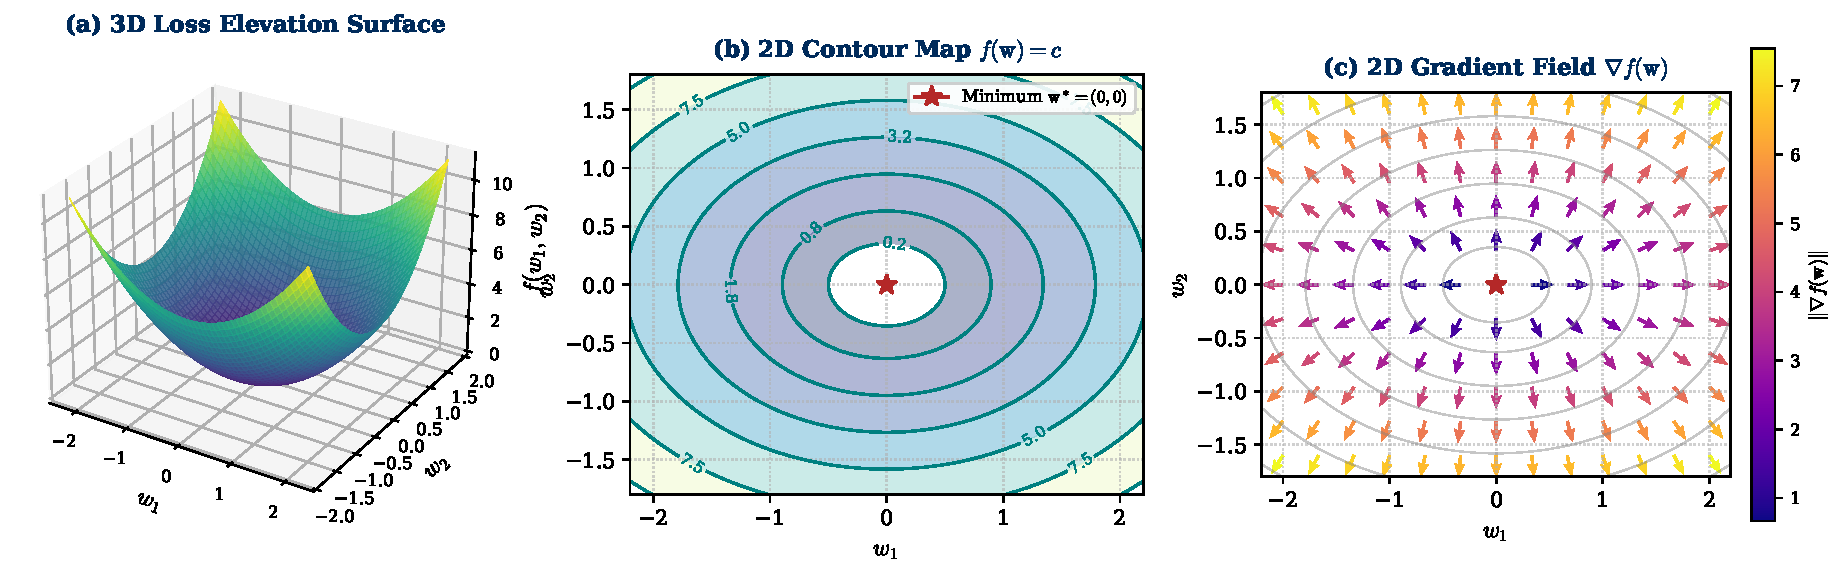
\includegraphics[width=\linewidth]{figures/gd_landscape_3panels.pdf}
\caption{Three synchronized representations of an optimization landscape $f(x, y)$: (Left) 3D surface plot displaying elevation peaks, valleys, and saddle regions; (Middle) 2D contour map showing level curves $f(x, y) = c$, where concentric closed loops enclose local minima or maxima; (Right) 2D vector field of gradients, where vector lengths indicate slope magnitude and arrows point in the direction of steepest ascent.}
\label{fig:gd_landscape_3panels}
\end{figure}

As displayed in Figure~\ref{fig:gd_landscape_3panels}:
\begin{enumerate}
  \item \textbf{3D Surface Plot (Elevation)}: Directly graphs the scalar cost value $z = f(x, y)$ as a function of the two parameters. Elevation reflects loss magnitude; global and local minima correspond to valleys.
  \item \textbf{2D Contour Map (Level Curves)}: Slices the 3D surface horizontally at constant loss elevations $f(x, y) = c$. Concentric closed isocurves enclose local extrema (minima or maxima). Spacing between contour lines indicates steepness: densely packed contours signify precipitous cliffs, whereas widely spaced contours indicate flat plateaus.
  \item \textbf{2D Gradient Vector Field}: Maps every coordinate $(x, y)$ to its gradient vector $\nabla f(x, y) = [\frac{\partial f}{\partial x}, \frac{\partial f}{\partial y}]^\top$. The arrows point in the direction of maximum instantaneous ascent, and their lengths represent the magnitude of the slope $\|\nabla f\|$.
\end{enumerate}

\subsection{Mathematical foundations: Differentiability and level curve orthogonality}
\label{sec:differentiability_and_orthogonality}

Before executing gradient updates, we must formalize two foundational mathematical principles emphasized in the AML curriculum:

\paragraph{1. The Differentiability Condition: Partial derivatives vs. true differentiability.}
Gradient descent updates require the objective function $f: \R^d \to \R$ to be differentiable. A frequent trap in mathematical analysis and oral examinations is confusing the existence of partial derivatives with true differentiability:
\begin{examinsight}[Oral Exam Pitfall: Differentiability vs. Partial Derivatives]
\textbf{The existence of all partial derivatives (or even all directional derivatives) does NOT imply that a function is differentiable!}\\
A multivariable function $f: \R^d \to \R$ is differentiable at $\mathbf{x}_0$ if and only if there exists a linear map (the gradient $\nabla f(\mathbf{x}_0)$) such that:
\begin{equation}
\lim_{\mathbf{h} \to \mathbf{0}} \frac{f(\mathbf{x}_0 + \mathbf{h}) - f(\mathbf{x}_0) - \nabla f(\mathbf{x}_0)^\top \mathbf{h}}{\|\mathbf{h}\|_2} = 0.
\label{eq:frechet_differentiability}
\end{equation}
By the Total Differential Theorem, a sufficient condition for differentiability is that all partial derivatives exist and are \textbf{continuous} ($f \in C^1$). If partial derivatives exist but are discontinuous, the function may fail to be differentiable, causing gradient descent to fail.
\end{examinsight}

To understand this distinction concretely, consider the classic counterexample:
\begin{equation}
f(x, y) = \begin{cases} 0 & \text{at } (x, y) = (0, 0), \\ \dfrac{x^2 y}{x^2 + y^2} & \text{elsewhere}. \end{cases}
\label{eq:differentiability_counterexample}
\end{equation}

\begin{figure}[htbp]
\centering
\begin{minipage}{0.48\linewidth}
  \centering
  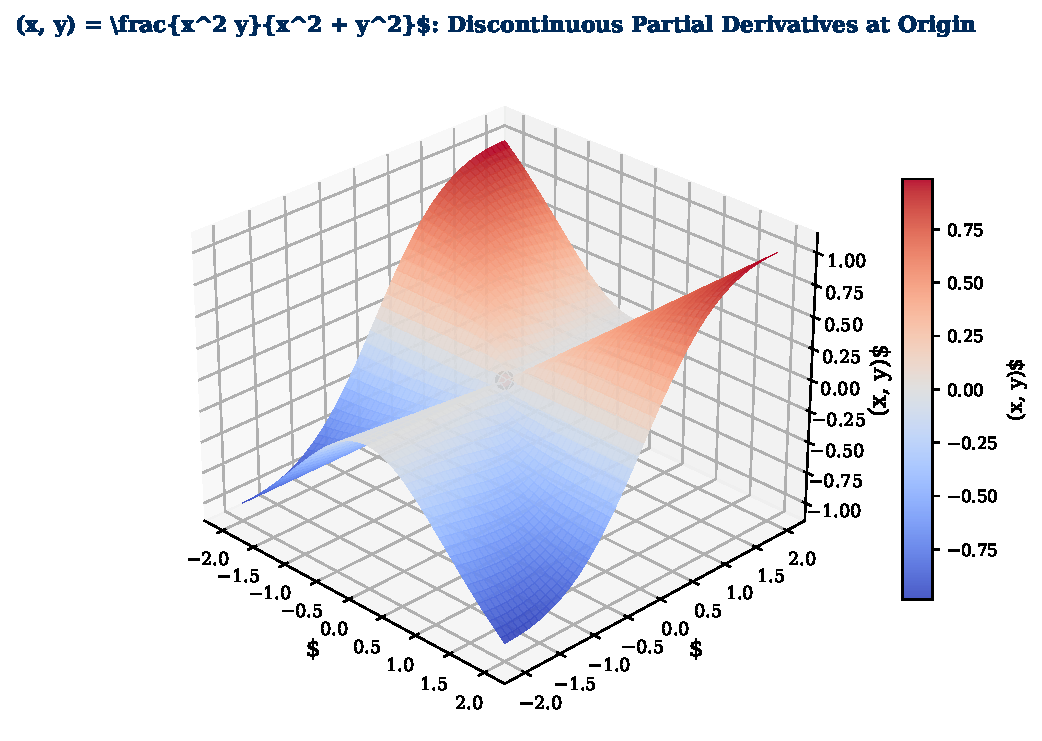
\includegraphics[width=0.95\linewidth]{figures/differentiability_counterexample_3d.pdf}
  \caption{3D surface plot of the counterexample function $f(x, y) = \frac{x^2 y}{x^2 + y^2}$ around the origin. Although partial derivatives exist everywhere, they are discontinuous at $(0, 0)$, rendering the surface non-differentiable.}
  \label{fig:differentiability_counterexample_3d}
\end{minipage}\hfill
\begin{minipage}{0.48\linewidth}
  \centering
  \begin{tikzpicture}[>=Stealth, scale=0.72, every node/.style={transform shape}]
    % Concentric elliptical contours of f(x,y)
    \draw[thick, gray!50] (0,0) ellipse (0.8cm and 0.5cm);
    \node[font=\tiny, gray!70] at (0, 0.6) {$f=0.5$};

    \draw[thick, deepdiveTeal!60] (0,0) ellipse (1.6cm and 1.0cm);
    \node[font=\tiny, deepdiveTeal!80] at (0, 1.15) {$f=1.5$};

    \draw[very thick, politoNavy] (0,0) ellipse (2.6cm and 1.6cm);
    \node[font=\scriptsize\bfseries, politoNavy] at (0, 1.8) {$\mathcal{C}_c: f(\mathbf{w}) = 2.5$};

    \draw[thick, gray!50] (0,0) ellipse (3.6cm and 2.2cm);
    \node[font=\tiny, gray!70] at (0, 2.4) {$f=4.0$};

    \draw[thick, gray!40] (0,0) ellipse (4.6cm and 2.8cm);
    \node[font=\tiny, gray!60] at (0, 3.0) {$f=6.0$};

    % Center minimum
    \fill[examred] (0,0) circle (2.5pt);
    \node[below=2pt, font=\scriptsize\bfseries, text=examred] at (0,0) {$\mathbf{w}^*$};

    % Marked point on level curve
    \coordinate (P) at (1.99, 1.03);
    \fill[politoNavy] (P) circle (3pt);
    \node[below left=2pt, font=\footnotesize\bfseries, text=politoNavy] at (P) {$\mathbf{w}_0$};

    % Tangent space line
    \draw[thick, dashed, gray!80] ($(P) + (1.61, -1.19)$) -- ($(P) + (-2.01, 1.48)$)
      node[above left, font=\scriptsize\bfseries, text=gray!90] {$\mathcal{T}_{\mathbf{w}_0}$};

    % Tangent vector v arrow
    \draw[->, very thick, deepdiveTeal] (P) -- ($(P) + (-1.21, 0.89)$)
      node[above, font=\footnotesize\bfseries, text=deepdiveTeal] {$\mathbf{v}$ ($df = 0$)};

    % Gradient vector: normal to tangent
    \draw[->, line width=1.6pt, examred] (P) -- ($(P) + (1.07, 1.45)$)
      node[above right, font=\footnotesize\bfseries, text=examred, align=left] {$\nabla f(\mathbf{w}_0)$};

    % Downhill negative gradient arrow
    \draw[->, line width=1.6pt, intuitiongreen] (P) -- ($(P) + (-1.07, -1.45)$)
      node[below right, font=\footnotesize\bfseries, text=intuitiongreen, align=left] {$-\nabla f(\mathbf{w}_0)$};

    % Right angle symbol
    \coordinate (RA1) at ($(P) + 0.28*(-0.805, 0.593)$);
    \coordinate (RA2) at ($(P) + 0.28*(-0.805, 0.593) + 0.28*(0.593, 0.805)$);
    \coordinate (RA3) at ($(P) + 0.28*(0.593, 0.805)$);
    \draw[thick, examred] (RA1) -- (RA2) -- (RA3);

    % Theorem callout
    \node[draw=politoNavy!70, fill=white, rounded corners=3pt, inner sep=3pt, font=\tiny, align=left] at (-1.8, -1.9) {
      $\langle \nabla f(\mathbf{w}_0), \mathbf{v} \rangle = 0 \quad \forall \mathbf{v} \in \mathcal{T}_{\mathbf{w}_0}$\\
      $\implies \nabla f \perp \text{Level Curves}$
    };
  \end{tikzpicture}
  \caption{Geometric orthogonality of the gradient to contour level curves. Along the isocurve $f(x, y) = 2.5$, the directional derivative along any tangent vector $\mathbf{v}$ is zero ($\langle \nabla f, \mathbf{v} \rangle = 0$). The negative gradient $-\nabla f$ points strictly perpendicular to the level curve in the direction of steepest descent.}
  \label{fig:gradient_orthogonal_level_curves}
\end{minipage}
\end{figure}

Evaluating the partial derivatives of Equation~\eqref{eq:differentiability_counterexample} at the coordinate origin via the difference quotient:
\begin{align}
\frac{\partial f}{\partial x}(0, 0) &= \lim_{h \to 0} \frac{f(h, 0) - f(0, 0)}{h} = \lim_{h \to 0} \frac{0 - 0}{h} = 0, \\
\frac{\partial f}{\partial y}(0, 0) &= \lim_{h \to 0} \frac{f(0, h) - f(0, 0)}{h} = \lim_{h \to 0} \frac{0 - 0}{h} = 0.
\end{align}
Both partial derivatives exist and equal zero at the origin. However, computing the partial derivative with respect to $y$ along the line $y = 0$ for any $x \ne 0$:
\begin{equation}
\frac{\partial f}{\partial y}(x, 0) = \left. \frac{x^2(x^2 + y^2) - x^2 y(2y)}{(x^2 + y^2)^2} \right|_{y=0} = \frac{x^4}{x^4} = 1.
\end{equation}
Meanwhile, along the $y$-axis ($x = 0$): $\frac{\partial f}{\partial y}(0, y) = 0$. Therefore, $\lim_{(x, y) \to (0, 0)} \frac{\partial f}{\partial y}(x, y)$ does not exist! The partial derivative is \textbf{discontinuous at the origin}, proving that $f(x, y)$ is not differentiable at $(0, 0)$, despite all directional derivatives being well-defined.

\paragraph{2. Orthogonality of the gradient to level curves.}
A second foundational geometric theorem is that the gradient vector is strictly \textbf{orthogonal} to the contour level curves (or level hypersurfaces in higher dimensions).

Let $\mathcal{C}_c \triangleq \{ \mathbf{w} \in \R^d : f(\mathbf{w}) = c \}$ be an isocurve of constant value $c$. Let $\mathbf{r}(t)$ be an arbitrary smooth path lying entirely within the level set, such that $f(\mathbf{r}(t)) = c$ for all $t$. Differentiating both sides with respect to scalar parameter $t$ via the multivariate chain rule:
\begin{equation}
\frac{d}{dt} f(\mathbf{r}(t)) = \nabla f(\mathbf{r}(t))^\top \mathbf{r}'(t) = 0.
\label{eq:level_curve_orthogonality_proof}
\end{equation}
Here, $\mathbf{r}'(t) \equiv \mathbf{v}$ is the tangent velocity vector along the contour curve. Equation~\eqref{eq:level_curve_orthogonality_proof} proves that:
\begin{equation}
\langle \nabla f(\mathbf{w}), \mathbf{v} \rangle = 0 \quad \text{for any tangent vector } \mathbf{v} \text{ to the isocurve}.
\end{equation}
Because the inner product vanishes, the directional derivative along the isocurve is zero: moving tangentially to a level set produces zero instantaneous change in loss. 

Conversely, the direction perpendicular to the tangent space maximizes the inner product, proving that the gradient vector $\nabla f(\mathbf{w})$ is \textbf{perpendicular to the level curves}, pointing toward steepest ascent, while the negative gradient $-\nabla f(\mathbf{w})$ points perpendicular to the level curves toward steepest descent (as illustrated in Figure~\ref{fig:gradient_orthogonal_level_curves}).

\subsection{Stationary points and initialization sensitivity}
\label{sec:stationary_points_initialization}

A point $\mathbf{x}^* \in \R^d$ where the gradient vanishes identically is defined as a \textbf{stationary point} (or critical point):
\begin{equation}
\nabla f(\mathbf{x}^*) = \mathbf{0}.
\label{eq:stationary_point_def}
\end{equation}
Evaluating the gradient descent update rule at a stationary point reveals an immediate consequence:
\begin{equation}
\mathbf{x}^{(t+1)} = \mathbf{x}^{(t)} - \alpha \nabla f(\mathbf{x}^{(t)}) = \mathbf{x}^{(t)} - \mathbf{0} = \mathbf{x}^{(t)}.
\end{equation}
Standard first-order gradient descent \textbf{gets stuck} at any stationary point, terminating all parameter updates.

However, a fundamental distinction must be drawn:
\begin{equation}
\text{Stationary Point } (\nabla f = \mathbf{0}) \quad \not\implies \quad \text{Local Minimum!}
\end{equation}
A stationary point can be a local minimum, a local maximum, or a saddle point. 

\begin{figure}[htbp]
\centering
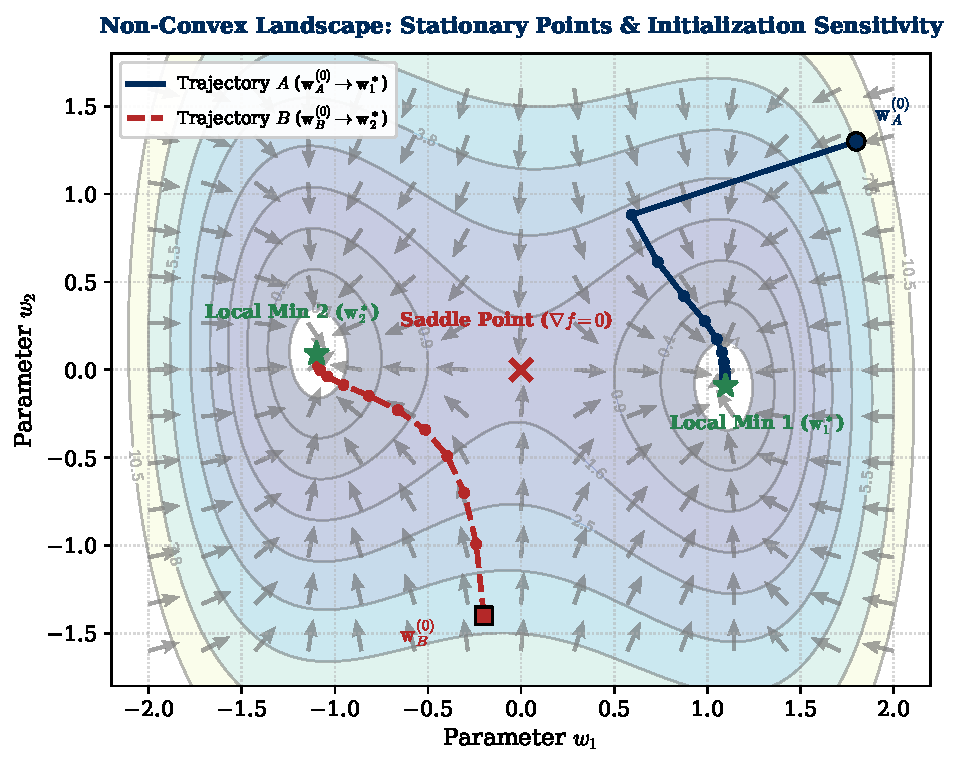
\includegraphics[width=0.55\linewidth]{figures/gd_trajectories_initialization.pdf}
\caption{Optimization trajectories on a non-convex vector field from different parameter initializations. Starting from the upper-right point, gradient updates follow the negative gradient arrows directly into a local minimum basin. Starting from the lower-left point, updates diverge along a completely different path toward a saddle region or alternative basin.}
\label{fig:gd_trajectories_initialization}
\end{figure}

As visualized in Figure~\ref{fig:gd_trajectories_initialization}, which stationary point gradient descent reaches depends entirely on the initial parameter configuration $\mathbf{x}^{(0)}$. In complex non-convex landscapes, different initializations lead to vastly different local basins or saddle geometries.

\subsection{Directional derivative and the proof of steepest descent}
\label{sec:directional_derivative_proof}

To formalize gradient descent from first principles, we analyze how a multivariate function changes along arbitrary spatial trajectories.

Let $f: \R^d \to \R$ be continuously differentiable ($C^1$). Let $\mathbf{u} \in \R^d$ be an arbitrary unit direction vector ($\|\mathbf{u}\|_2 = 1$). The \textbf{directional derivative} of $f$ at point $\mathbf{w}$ along direction $\mathbf{u}$ is defined as the limit:
\begin{equation}
D_\mathbf{u} f(\mathbf{w}) = \lim_{\epsilon \to 0} \frac{f(\mathbf{w} + \epsilon \mathbf{u}) - f(\mathbf{w})}{\epsilon}.
\label{eq:directional_derivative_def}
\end{equation}
By multivariable Taylor theorem, expanding $f(\mathbf{w} + \epsilon \mathbf{u})$ around $\mathbf{w}$:
\begin{equation}
f(\mathbf{w} + \epsilon \mathbf{u}) = f(\mathbf{w}) + \epsilon \nabla f(\mathbf{w})^\top \mathbf{u} + \mathcal{O}(\epsilon^2).
\end{equation}
Substituting this expansion into Equation~\eqref{eq:directional_derivative_def}:
\begin{equation}
D_\mathbf{u} f(\mathbf{w}) = \lim_{\epsilon \to 0} \frac{\epsilon \nabla f(\mathbf{w})^\top \mathbf{u} + \mathcal{O}(\epsilon^2)}{\epsilon} = \nabla f(\mathbf{w})^\top \mathbf{u}.
\label{eq:directional_derivative_inner_product}
\end{equation}
The rate of change along direction $\mathbf{u}$ is given by the inner product of the gradient vector $\nabla f(\mathbf{w})$ with $\mathbf{u}$.

To minimize $f(\mathbf{w})$, we seek the unit direction $\mathbf{u}^*$ that minimizes the directional derivative (i.e., maximizes the rate of instantaneous decrease):
\begin{equation}
\mathbf{u}^* = \arg\min_{\|\mathbf{u}\|_2 = 1} D_\mathbf{u} f(\mathbf{w}) = \arg\min_{\|\mathbf{u}\|_2 = 1} \nabla f(\mathbf{w})^\top \mathbf{u}.
\label{eq:steepest_descent_problem}
\end{equation}
By the Cauchy-Schwarz inequality, for any two vectors $\mathbf{a}, \mathbf{b} \in \R^d$:
\begin{equation}
|\mathbf{a}^\top \mathbf{b}| \le \|\mathbf{a}\|_2 \|\mathbf{b}\|_2 \implies -\sum_{j=1}^d a_j b_j \ge -\|\mathbf{a}\|_2 \|\mathbf{b}\|_2.
\end{equation}
Applying this bound to Equation~\eqref{eq:steepest_descent_problem} with $\mathbf{a} = \nabla f(\mathbf{w})$ and $\mathbf{b} = \mathbf{u}$ (where $\|\mathbf{u}\|_2 = 1$):
\begin{equation}
\nabla f(\mathbf{w})^\top \mathbf{u} \ge -\|\nabla f(\mathbf{w})\|_2 \|\mathbf{u}\|_2 = -\|\nabla f(\mathbf{w})\|_2.
\label{eq:cauchy_schwarz_lower_bound}
\end{equation}
Equality holds if and only if vector $\mathbf{u}$ is collinear with $\nabla f(\mathbf{w})$ and points in the opposite direction:
\begin{equation}
\mathbf{u}^* = -\frac{\nabla f(\mathbf{w})}{\|\nabla f(\mathbf{w})\|_2}.
\label{eq:steepest_descent_direction}
\end{equation}
This rigorous derivation proves Cauchy's 1847 theorem~\cite{cauchy1847methode}: \textbf{the negative gradient direction $-\nabla f(\mathbf{w})$ is the direction of steepest instantaneous descent}.

Geometrically, because $\nabla f(\mathbf{w})$ is strictly perpendicular to the level curves of a continuous surface, stepping along $-\nabla f(\mathbf{w})$ guarantees maximum loss reduction per unit distance moved in high-dimensional spaces.

\subsection{First-order Taylor expansion and the gradient descent update}
\label{sec:first_order_taylor}

We parameterize a finite step of length $\eta > 0$ along direction $\mathbf{u}^*$, yielding displacement $\Delta \mathbf{w} = -\eta \nabla f(\mathbf{w})$. The first-order Taylor series approximation around point $\mathbf{w}_t$ is:
\begin{equation}
f(\mathbf{w}_t - \eta \nabla f(\mathbf{w}_t)) \approx f(\mathbf{w}_t) - \eta \|\nabla f(\mathbf{w}_t)\|_2^2 + \mathcal{O}(\eta^2).
\label{eq:taylor_first_order}
\end{equation}
Because $\|\nabla f(\mathbf{w}_t)\|_2^2 > 0$ for any non-stationary point, there exists a sufficiently small step size $\eta > 0$ such that the second-order remainder is dominated by the linear decrease:
\begin{equation}
f(\mathbf{w}_t - \eta \nabla f(\mathbf{w}_t)) < f(\mathbf{w}_t).
\end{equation}
This establishes the classical \textbf{Gradient Descent update rule}:
\begin{equation}
\mathbf{w}_{t+1} = \mathbf{w}_t - \eta \nabla f(\mathbf{w}_t),
\label{eq:gradient_descent_update}
\end{equation}
where $\eta > 0$ is the \textbf{learning rate} (step size hyperparameter).

\subsection{Learning rate dynamics: Under-stepping vs. divergence}
\label{sec:learning_rate_dynamics}

The magnitude of the learning rate $\eta$ critically dictates optimization stability:

\begin{figure}[htbp]
\centering
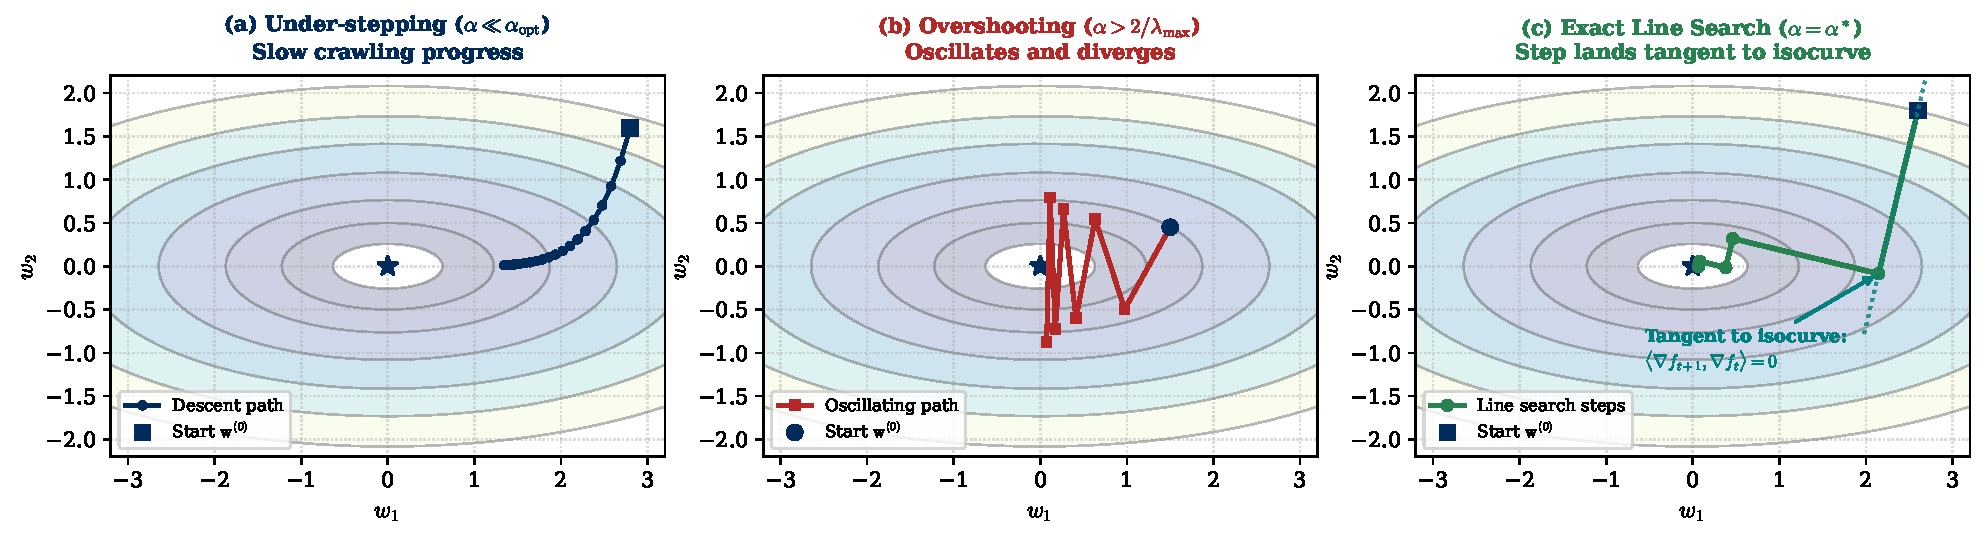
\includegraphics[width=\linewidth]{figures/learning_rate_dynamics_contours.pdf}
\caption{Contour dynamics of gradient descent under varying step sizes $\alpha$: (Left) An excessively small learning rate causes crawling, agonizingly slow progress along the contour gradient; (Middle) An excessively large learning rate overshoots the minimum, oscillating across valley walls with increasing amplitude and ultimately diverging; (Right) An optimal step size determined via line search $\arg\min_\alpha f(\mathbf{x}^{(t)} - \alpha \nabla f(\mathbf{x}^{(t)}))$, where each update lands precisely where the descent direction is tangent to a contour isocurve.}
\label{fig:slide_learning_rates}
\end{figure}

As illustrated across the contour landscapes in Figure~\ref{fig:slide_learning_rates}:
\begin{itemize}
  \item \textbf{Effective Step Length}: An essential mathematical nuance is that the geometric length of the parameter update is not simply the scalar learning rate $\alpha$, but rather the norm-scaled quantity $\alpha \|\nabla f(\mathbf{x}^{(t)})\|$. In regions where the gradient is steep, the parameter displacement is proportionally magnified; conversely, on shallow plateaus where $\|\nabla f\| \approx 0$, progress stalls regardless of $\alpha$.
  \item \textbf{Under-stepping ($\alpha \to 0$)}: When $\alpha$ is excessively conservative, parameter updates $\Delta \mathbf{x}^{(t)}$ are microscopic. Iterations advance imperceptibly, requiring thousands of steps to cross moderate distances and rendering the optimizer vulnerable to premature convergence on deceptive plateaus.
  \item \textbf{Overshooting and Divergence ($\alpha \gg \alpha_{\text{crit}}$)}: When $\alpha$ exceeds the critical threshold dictated by the maximum eigenvalue of the Hessian ($\alpha > 2/\lambda_{\max}$, proven in Section~\ref{sec:condition_number_ravines}), the first-order Taylor approximation breaks down completely. Updates violently oscillate back and forth between opposing valley walls with geometrically increasing amplitude, driving objective values toward infinity: $\lim_{t \to \infty} f(\mathbf{x}^{(t)}) = \infty$.
  \item \textbf{Optimal Step Size via Exact Line Search}: In classical optimization, the optimal step size is determined adaptively by solving a one-dimensional sub-problem along the negative gradient ray:
    \begin{equation}
    \alpha^* = \arg\min_{\alpha > 0} f\left(\mathbf{x}^{(t)} - \alpha \nabla f(\mathbf{x}^{(t)})\right).
    \label{eq:exact_line_search}
    \end{equation}
    Evaluating the optimality condition by differentiating with respect to $\alpha$ via the multivariate chain rule:
    \begin{equation}
    \frac{d}{d\alpha} f\left(\mathbf{x}^{(t)} - \alpha \nabla f(\mathbf{x}^{(t)})\right) = -\nabla f\left(\mathbf{x}^{(t+1)}\right)^\top \nabla f\left(\mathbf{x}^{(t)}\right) = 0.
    \label{eq:line_search_orthogonality}
    \end{equation}
    Equation~\eqref{eq:line_search_orthogonality} reveals a fundamental geometric theorem: at the exact line-search minimizer, the new gradient $\nabla f(\mathbf{x}^{(t+1)})$ is strictly perpendicular to the previous search direction $-\nabla f(\mathbf{x}^{(t)})$. In terms of contour topology, this means the gradient direction at the landing point is \textbf{tangent to the local isocurve} (level set), producing the characteristic orthogonal zig-zag trajectory shown in the right panel of Figure~\ref{fig:slide_learning_rates}.
\end{itemize}

\subsection{Learning rate decay schedules: Linear, inverse, and exponential}
\label{sec:learning_rate_decay_schedules}

Fixing a constant scalar learning rate $\alpha$ forces an undesirable trade-off: a large learning rate enables rapid traversal of distant plateaus early in training but prevents convergence near the minimum due to endless cross-valley oscillations; conversely, a small learning rate ensures stable fine-grained convergence but crawls agonizingly slowly at initialization.

To reconcile these competing objectives, the learning rate can be modulated dynamically over iterations according to a deterministic \textbf{decay schedule} parameterized by a decay factor $\rho > 0$:

\paragraph{1. Linear decay schedule.}
The linear decay schedule interpolates parameter updates uniformly from an initial step size $\alpha^{(0)}$ down to a designated final floor $\alpha^{(\rho)}$ over a budget of $\rho$ iterations:
\begin{equation}
\alpha^{(t+1)} = \left(1 - \frac{t}{\rho}\right)\alpha^{(0)} + \frac{t}{\rho}\alpha^{(\rho)}, \quad \text{for } 0 \le t \le \rho.
\label{eq:linear_decay_schedule}
\end{equation}
At iteration $t = 0$, $\alpha^{(1)} = \alpha^{(0)}$. At the terminal horizon $t = \rho$, the learning rate contracts precisely to $\alpha^{(\rho)}$ (typically chosen orders of magnitude smaller than $\alpha^{(0)}$). For iterations $t > \rho$, the rate remains fixed at $\alpha^{(\rho)}$. This schedule provides predictable, constant-rate deceleration.

\paragraph{2. Inverse decay schedule (Time-based decay).}
The inverse decay schedule attenuates the step size inversely with the elapsed iteration count:
\begin{equation}
\alpha^{(t+1)} = \frac{\alpha^{(t)}}{1 + \rho t}.
\label{eq:inverse_decay_schedule}
\end{equation}
In its direct non-recursive formulation, $\alpha^{(t)} = \frac{\alpha^{(0)}}{1 + \rho t}$. This schedule enforces an asymptotic decay rate of $\mathcal{O}(1/t)$, mirroring the classical Robbins-Monro stochastic convergence rate (detailed in Section~\ref{sec:robbins_monro}) while ensuring rapid initial dampening that smoothly transitions into a long-tailed fine-tuning regime.

\paragraph{3. Exponential decay schedule.}
The exponential decay schedule applies continuous geometric dampening scaled by decay rate $\rho > 0$:
\begin{equation}
\alpha^{(t+1)} = \alpha^{(0)} e^{-\rho t}.
\label{eq:exponential_decay_schedule}
\end{equation}
Because the step size contracts by a constant multiplicative factor $e^{-\rho}$ at every iteration, exponential decay rapidly quenches parameter updates. In contemporary deep learning practice, this is frequently discretized into \emph{step decay} (e.g., decaying $\alpha$ by a factor of $0.1$ or $0.2$ every fixed number of epochs).

---

\section{Second-order curvature, the Hessian matrix, and ill-conditioned ravines}
\label{sec:second_order_curvature}

First-order gradient descent operates under the implicit assumption that the surface is locally linear. However, when the loss surface exhibits high curvature, second derivatives dominate optimization trajectories.

\subsection{The Hessian matrix and second-order Taylor expansion}
\label{sec:hessian_matrix}

Let $f: \R^d \to \R$ be twice continuously differentiable ($C^2$). The second-order Taylor series approximation of $f$ around point $\mathbf{w}$ for an arbitrary displacement $\Delta \mathbf{w} \in \R^d$ is:
\begin{equation}
f(\mathbf{w} + \Delta \mathbf{w}) \approx f(\mathbf{w}) + \nabla f(\mathbf{w})^\top \Delta \mathbf{w} + \frac{1}{2} \Delta \mathbf{w}^\top \mathbf{H}(\mathbf{w}) \Delta \mathbf{w},
\label{eq:second_order_taylor}
\end{equation}
where $\mathbf{H}(\mathbf{w}) \in \R^{d \times d}$ is the \textbf{Hessian matrix} of second-order partial derivatives:
\begin{equation}
\mathbf{H}_{jk}(\mathbf{w}) = \frac{\partial^2 f(\mathbf{w})}{\partial w_j \partial w_k}, \quad j, k \in \{1, \dots, d\}.
\label{eq:hessian_def}
\end{equation}
By Schwarz's theorem on the equality of mixed partials, $\frac{\partial^2 f}{\partial w_j \partial w_k} = \frac{\partial^2 f}{\partial w_k \partial w_j}$, guaranteeing that $\mathbf{H}$ is a real symmetric matrix ($\mathbf{H} = \mathbf{H}^\top$).

By the spectral theorem, the symmetric Hessian admits an orthogonal eigendecomposition:
\begin{equation}
\mathbf{H} = \mathbf{Q} \mathbf{\Lambda} \mathbf{Q}^\top = \sum_{i=1}^d \lambda_i \mathbf{q}_i \mathbf{q}_i^\top,
\label{eq:hessian_spectral}
\end{equation}
where $\mathbf{Q} = [\mathbf{q}_1, \dots, \mathbf{q}_d] \in \R^{d \times d}$ is an orthonormal matrix of eigenvectors ($\mathbf{q}_i^\top \mathbf{q}_j = \delta_{ij}$), and $\mathbf{\Lambda} = \operatorname{diag}(\lambda_1, \dots, \lambda_d)$ contains real eigenvalues ordered such that $\lambda_{\max} \equiv \lambda_1 \ge \lambda_2 \ge \dots \ge \lambda_d \equiv \lambda_{\min}$.

The quadratic term $\frac{1}{2} \Delta \mathbf{w}^\top \mathbf{H} \Delta \mathbf{w}$ characterizes directional curvature:
\begin{itemize}[noitemsep]
  \item If $\Delta \mathbf{w}$ aligns with eigenvector $\mathbf{q}_i$, the second-order change is $\frac{1}{2} \lambda_i \|\Delta \mathbf{w}\|_2^2$.
  \item A positive eigenvalue ($\lambda_i > 0$) signifies positive curvature (the function curves upward like a bowl).
  \item A negative eigenvalue ($\lambda_i < 0$) signifies negative curvature (the function curves downward like a dome).
  \item A zero eigenvalue ($\lambda_i = 0$) signifies flat curvature (the function is locally linear along $\mathbf{q}_i$).
\end{itemize}

\paragraph{Optimal step size under second-order curvature.}
Substituting the gradient descent step $\Delta \mathbf{w} = -\eta \mathbf{g}$ (where $\mathbf{g} = \nabla f(\mathbf{w})$) into Equation~\eqref{eq:second_order_taylor}:
\begin{equation}
f(\mathbf{w} - \eta \mathbf{g}) \approx f(\mathbf{w}) - \eta \mathbf{g}^\top \mathbf{g} + \frac{1}{2} \eta^2 \mathbf{g}^\top \mathbf{H} \mathbf{g}.
\label{eq:gd_step_taylor2}
\end{equation}
To find the step size $\eta^*$ that maximizes expected decrease, we differentiate Equation~\eqref{eq:gd_step_taylor2} with respect to scalar $\eta$ and set the derivative to zero:
\begin{equation}
\frac{d}{d\eta} \left[ f(\mathbf{w}) - \eta \|\mathbf{g}\|_2^2 + \frac{1}{2} \eta^2 \mathbf{g}^\top \mathbf{H} \mathbf{g} \right] = -\|\mathbf{g}\|_2^2 + \eta \mathbf{g}^\top \mathbf{H} \mathbf{g} = 0 \implies \eta^* = \frac{\mathbf{g}^\top \mathbf{g}}{\mathbf{g}^\top \mathbf{H} \mathbf{g}}.
\label{eq:optimal_eta_hessian}
\end{equation}
If the gradient vector happens to align with the dominant eigenvector of the Hessian ($\mathbf{g} \approx \mathbf{q}_1$), the optimal learning rate contracts to $\eta^* = 1/\lambda_{\max}$. Moreover, convergence requires:
\begin{equation}
0 < \eta < \frac{2}{\lambda_{\max}(\mathbf{H})}.
\label{eq:learning_rate_stability_bound}
\end{equation}
If $\eta \ge 2/\lambda_{\max}$, the quadratic term exceeds the linear decrease, and the iterates diverge.

\subsection{The condition number and ill-conditioned ravines}
\label{sec:condition_number_ravines}

A fundamental computational bottleneck for first-order gradient descent is the phenomenon of \textbf{ill-conditioned ravines} (also known as valleys or canyons).

\begin{definition}[Hessian condition number]
For a convex objective with positive definite Hessian ($\mathbf{H} \succ 0$, so all $\lambda_i > 0$), the \textbf{condition number} $\kappa \ge 1$ is defined as the ratio of maximum to minimum eigenvalue:
\begin{equation}
\kappa(\mathbf{H}) = \frac{\lambda_{\max}(\mathbf{H})}{\lambda_{\min}(\mathbf{H})}.
\label{eq:condition_number_def}
\end{equation}
\end{definition}

When $\kappa \approx 1$, the contour lines of the loss surface are isotropic hyperspheres. The gradient vector points directly toward the minimum, and gradient descent converges rapidly.

However, when $\kappa \gg 1$ (e.g., $\kappa = 10^3$ or $10^5$), the problem is termed \textbf{ill-conditioned}. The contour lines form elongated, highly eccentric ellipsoids.

\begin{figure}[htbp]
\centering
\begin{minipage}{0.48\linewidth}
  \centering
  \begin{tikzpicture}[scale=0.68, every node/.style={transform shape}]
    % Axes
    \draw[-{Stealth}, gray!60, thick] (-3.8, 0) -- (4.0, 0) node[right, font=\footnotesize] {$\mathbf{q}_2$ ($\lambda_{\min}$)};
    \draw[-{Stealth}, gray!60, thick] (0, -2.0) -- (0, 2.0) node[above, font=\footnotesize] {$\mathbf{q}_1$ ($\lambda_{\max}$)};

    % Contours
    \draw[politoNavy!35, thick] (0, 0) ellipse (3.5 and 1.6);
    \draw[politoNavy!55, thick] (0, 0) ellipse (2.7 and 1.15);
    \draw[politoNavy!75, thick] (0, 0) ellipse (1.9 and 0.75);
    \draw[politoNavy!90, thick] (0, 0) ellipse (1.2 and 0.4);
    \draw[politoNavy, thick] (0, 0) ellipse (0.5 and 0.15);

    % Minimizer
    \node[star, star points=5, star point ratio=2.25, fill=intuitiongreen, inner sep=2pt, label={below left:\scriptsize $\mathbf{w}^*$}] at (0, 0) {};

    % Trajectory
    \coordinate (p0) at (3.1, 1.35);
    \coordinate (p1) at (2.8, -1.05);
    \coordinate (p2) at (2.5, 0.82);
    \coordinate (p3) at (2.2, -0.62);
    \coordinate (p4) at (1.9, 0.48);
    \coordinate (p5) at (1.6, -0.35);
    \coordinate (p6) at (1.3, 0.25);

    \draw[-{Stealth}, thick, examred] (p0) -- (p1);
    \draw[-{Stealth}, thick, examred] (p1) -- (p2);
    \draw[-{Stealth}, thick, examred] (p2) -- (p3);
    \draw[-{Stealth}, thick, examred] (p3) -- (p4);
    \draw[-{Stealth}, thick, examred] (p4) -- (p5);
    \draw[-{Stealth}, thick, examred] (p5) -- (p6);

    \foreach \p in {p0,p1,p2,p3,p4,p5,p6} {
      \fill[examred] (\p) circle (1.6pt);
    }
    \node[above right, font=\scriptsize\bfseries, text=examred] at (p0) {$\mathbf{w}_0$};

    \node[font=\scriptsize, text=examred, align=center] at (2.2, -1.6) {Cross-ravine\\oscillations};
    \node[font=\scriptsize, text=deepdiveTeal, align=center] at (-1.8, 1.2) {Slow progress\\along base};
  \end{tikzpicture}
\end{minipage}\hfill
\begin{minipage}{0.48\linewidth}
  \centering
  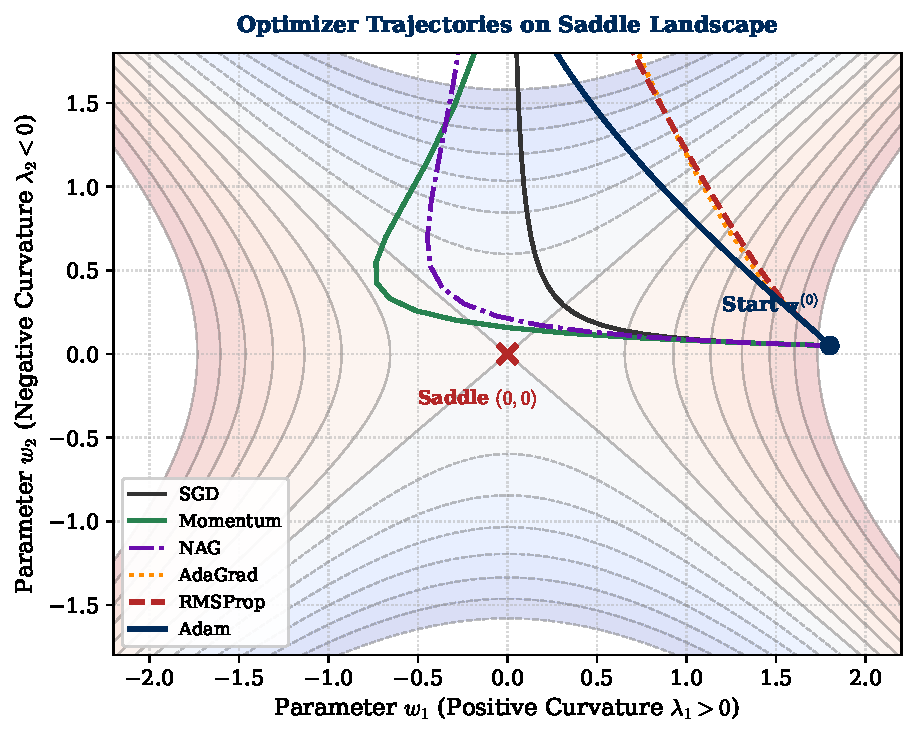
\includegraphics[width=\linewidth]{figures/cs231n_optimizer_comparison.pdf}
\end{minipage}
\caption{Optimization dynamics in ill-conditioned ravines and complex landscapes. Left: Native vector representation of an ill-conditioned quadratic valley ($\kappa = \lambda_{\max}/\lambda_{\min} \gg 1$), where first-order gradient descent oscillates violently across the steep walls along $\mathbf{q}_1$ while making negligible progress along the flat base $\mathbf{q}_2$. Right: Benchmark comparison across optimizers (SGD, Momentum, NAG, AdaGrad, AdaDelta, RMSProp) traversing a saddle topology, demonstrating how momentum and adaptive learning rates overcome anisotropic curvature.}
\label{fig:slide_ill_conditioned_ravine}
\end{figure}

As visualized in Figure~\ref{fig:slide_ill_conditioned_ravine}:
\begin{itemize}
  \item Along the direction of maximum curvature $\mathbf{q}_1$ (across the ravine walls), the loss changes rapidly with eigenvalue $\lambda_{\max}$.
  \item Along the direction of minimum curvature $\mathbf{q}_2$ (along the ravine base leading to the minimum), the loss changes extremely slowly with eigenvalue $\lambda_{\min}$.
  \item The stability bound in Equation~\eqref{eq:learning_rate_stability_bound} restricts the global learning rate to $\eta < 2/\lambda_{\max}$.
  \item Because $\eta$ must be chosen small to prevent explosive divergence across the steep walls, progress along the flat base is scaled by $\eta \lambda_{\min} < 2 \frac{\lambda_{\min}}{\lambda_{\max}} = \frac{2}{\kappa} \ll 1$.
\end{itemize}
Consequently, first-order gradient descent oscillates violently back and forth between the opposing walls of the ravine, making negligible forward progress toward the true minimizer.

This curvature imbalance causes standard first-order algorithms to stall in narrow ravines, providing the direct theoretical motivation for \textbf{Momentum} methods and \textbf{Adaptive Optimizers} (such as RMSProp and Adam~\cite{kingma2014adam}), which dampen cross-ravine oscillations while accumulating directional velocity along the base.

---

\section{First-order acceleration methods: Momentum and unified matrix scaling}
\label{sec:first_order_acceleration_methods}

As established in Section~\ref{sec:condition_number_ravines}, first-order gradient descent suffers from pathological oscillations in ill-conditioned ravines ($\kappa \gg 1$). To circumvent this bottleneck without incurring the prohibitive $\mathcal{O}(d^3)$ cost of explicit Hessian inversion, first-order optimization is augmented through \textbf{momentum} and \textbf{adaptive scaling}.

\subsection{Classical momentum: Velocity accumulation and oscillation dampening}
\label{sec:classical_momentum}

The classical momentum method, formulated by Boris Polyak in 1964~\cite{polyak1964some}, draws direct inspiration from physical mechanics. Rather than treating the parameter vector as a massless particle whose velocity instantly matches the local negative gradient, the optimizer models a heavy marble rolling down a frictioned potential well.

The algorithm introduces an internal state vector $\mathbf{v}^{(t)} \in \R^d$, termed the \textbf{velocity}, and updates parameters according to the coupled recurrence:
\begin{align}
\mathbf{v}^{(t+1)} &= \lambda \mathbf{v}^{(t)} - \alpha \nabla f(\mathbf{x}^{(t)}), \label{eq:momentum_velocity_update} \\
\mathbf{x}^{(t+1)} &= \mathbf{x}^{(t)} + \mathbf{v}^{(t+1)}, \label{eq:momentum_position_update}
\end{align}
where $\alpha > 0$ is the learning rate, and $\lambda \in [0, 1)$ is the \textbf{momentum coefficient} (or friction parameter, typically set to $\lambda = 0.9$ or $0.99$).

\paragraph{Physical mechanism in ill-conditioned valleys.}
When $\lambda = 0$, the velocity simplifies to $\mathbf{v}^{(t+1)} = -\alpha \nabla f(\mathbf{x}^{(t)})$, collapsing immediately to standard gradient descent. 
When $\lambda > 0$, the velocity retains an exponential moving average of historical gradient directions:
\begin{itemize}[noitemsep]
  \item \textbf{Transverse cross-ravine direction ($\mathbf{q}_1$)}: Because the optimizer repeatedly bounces back and forth across the opposing valley walls, the signs of consecutive partial derivatives alternate: $\nabla f(\mathbf{x}^{(t)})_{\mathbf{q}_1} \approx -\nabla f(\mathbf{x}^{(t-1)})_{\mathbf{q}_1}$. In the velocity accumulator of Equation~\eqref{eq:momentum_velocity_update}, these opposing vectors cancel out destructively:
  \begin{equation}
  \mathbf{v}^{(t+1)}_{\mathbf{q}_1} \approx \lambda \mathbf{v}^{(t)}_{\mathbf{q}_1} - \alpha \nabla f(\mathbf{x}^{(t)})_{\mathbf{q}_1} \approx \mathbf{0}.
  \end{equation}
  This destructive interference aggressively dampens high-frequency cross-ravine oscillations.
  \item \textbf{Longitudinal base direction ($\mathbf{q}_2$)}: Along the gentle descent floor of the valley leading toward the minimizer, consecutive gradients point consistently in the same downhill direction: $\nabla f(\mathbf{x}^{(t)})_{\mathbf{q}_2} \approx \nabla f(\mathbf{x}^{(t-1)})_{\mathbf{q}_2}$. Here, the historical velocity terms add constructively, accumulating directional speed along the base.
\end{itemize}

\subsection{Effective terminal step length and aligned gradient acceleration}
\label{sec:aligned_gradient_acceleration}

A central pedagogical result is quantifying the exact acceleration gain when gradients are persistently aligned.

Suppose the optimizer traverses a uniform slope where the gradient remains constant over consecutive iterations: $\nabla f(\mathbf{x}^{(t)}) \approx \mathbf{g}$. Assuming initial velocity $\mathbf{v}^{(0)} = \mathbf{0}$, unrolling the recurrence in Equation~\eqref{eq:momentum_velocity_update} yields:
\begin{align}
\mathbf{v}^{(1)} &= -\alpha \mathbf{g}, \nonumber \\
\mathbf{v}^{(2)} &= -\lambda \alpha \mathbf{g} - \alpha \mathbf{g} = -\alpha (1 + \lambda) \mathbf{g}, \nonumber \\
\mathbf{v}^{(3)} &= -\lambda \alpha (1 + \lambda) \mathbf{g} - \alpha \mathbf{g} = -\alpha (1 + \lambda + \lambda^2) \mathbf{g}, \nonumber \\
&\;\;\vdots \nonumber \\
\mathbf{v}^{(t+1)} &= -\alpha \mathbf{g} \sum_{k=0}^t \lambda^k.
\label{eq:momentum_geometric_series}
\end{align}
Because $\lambda \in [0, 1)$, the finite summation in Equation~\eqref{eq:momentum_geometric_series} is a geometric progression. Taking the limit as $t \to \infty$:
\begin{equation}
\lim_{t \to \infty} \sum_{k=0}^t \lambda^k = \frac{1}{1 - \lambda}.
\end{equation}
Consequently, the terminal velocity and effective parameter displacement per step converge to:
\begin{equation}
\lim_{t \to \infty} \|\mathbf{v}^{(t+1)}\| = \frac{1}{1 - \lambda} \alpha \|\mathbf{g}\| = \frac{1}{1 - \lambda} \alpha \|\nabla f\|.
\label{eq:terminal_momentum_step}
\end{equation}
Equation~\eqref{eq:terminal_momentum_step} reveals the remarkable speedup factor of momentum:
\begin{itemize}[noitemsep]
  \item For standard gradient descent, the step length along a flat plateau with gradient $\|\nabla f\|$ is strictly $\alpha \|\nabla f\|$.
  \item For momentum with $\lambda = 0.9$, the effective step length expands to $\frac{1}{1 - 0.9}\alpha \|\nabla f\| = \mathbf{10 \alpha \|\nabla f\|}$ ($10\times$ acceleration).
  \item For momentum with $\lambda = 0.99$, the effective step length expands to $\frac{1}{1 - 0.99}\alpha \|\nabla f\| = \mathbf{100 \alpha \|\nabla f\|}$ ($100\times$ acceleration).
\end{itemize}
This dynamic amplification enables momentum to surge rapidly through flat regions and provides the kinetic energy required to carry parameter updates over shallow local barriers into deeper, more generalizing minima basins.

\subsection{Mathematical unrolling: Standard gradient descent vs. momentum}
\label{sec:unrolling_gd_momentum}

To understand how momentum transforms optimization trajectories over an entire training run, we analyze the concept of \textbf{unrolling the optimization recurrence}.

\paragraph{Unrolling standard gradient descent.}
For standard gradient descent without momentum, parameter updates follow $\mathbf{x}^{(t+1)} = \mathbf{x}^{(t)} - \alpha \nabla f(\mathbf{x}^{(t)})$. Unrolling step by step from initialization $\mathbf{x}^{(0)}$:
\begin{align}
\mathbf{x}^{(1)} &= \mathbf{x}^{(0)} - \alpha \nabla f(\mathbf{x}^{(0)}), \nonumber \\
\mathbf{x}^{(2)} &= \mathbf{x}^{(1)} - \alpha \nabla f(\mathbf{x}^{(1)}) = \mathbf{x}^{(0)} - \alpha \nabla f(\mathbf{x}^{(0)}) - \alpha \nabla f(\mathbf{x}^{(1)}), \nonumber \\
&\;\;\vdots \nonumber \\
\mathbf{x}^{(t+1)} &= \mathbf{x}^{(0)} - \alpha \sum_{i=1}^t \nabla f(\mathbf{x}^{(i)}).
\label{eq:unrolled_gd}
\end{align}
Equation~\eqref{eq:unrolled_gd} shows that in standard gradient descent, the net parameter displacement $\mathbf{x}^{(t+1)} - \mathbf{x}^{(0)}$ is simply the unweighted sum of all historical gradients, multiplied by constant step size $-\alpha$. Every historical gradient receives identical weighting, regardless of whether it was computed at the start of training or in the current iteration.

\paragraph{Unrolling gradient descent with momentum.}
Now consider the momentum update defined by Equations~\eqref{eq:momentum_velocity_update}--\eqref{eq:momentum_position_update}. Assuming $\mathbf{v}^{(0)} = \mathbf{0}$, the velocity at any iteration $k \ge 1$ is an exponentially decayed sum of past gradients:
\begin{equation}
\mathbf{v}^{(k)} = -\alpha \sum_{j=1}^k \lambda^{k-j} \nabla f(\mathbf{x}^{(j-1)}).
\end{equation}
Since $\mathbf{x}^{(t+1)} = \mathbf{x}^{(0)} + \sum_{k=1}^{t+1} \mathbf{v}^{(k)}$, the cumulative displacement after $t+1$ steps is:
\begin{equation}
\mathbf{x}^{(t+1)} = \mathbf{x}^{(0)} - \alpha \sum_{k=1}^{t+1} \sum_{j=1}^k \lambda^{k-j} \nabla f(\mathbf{x}^{(j-1)}).
\end{equation}
To determine the net coefficient multiplying each individual gradient $\nabla f(\mathbf{x}^{(i)})$ (for $i = 1, \dots, t$), we observe how often $\nabla f(\mathbf{x}^{(i)})$ enters into subsequent velocity terms:
\begin{itemize}[noitemsep]
  \item At iteration $k = i+1$, $\nabla f(\mathbf{x}^{(i)})$ enters with weight $-\alpha \lambda^0 = -\alpha$.
  \item At iteration $k = i+2$, it persists decayed by $-\alpha \lambda^1$.
  \item At iteration $k = i+3$, it persists decayed by $-\alpha \lambda^2$.
  \item $\dots$
  \item At iteration $k = t+1$, it persists decayed by $-\alpha \lambda^{t-i}$.
\end{itemize}
Summing these contributions across all subsequent steps gives a finite geometric series of length $t - i + 1$:
\begin{equation}
\sum_{m=0}^{t-i} \lambda^m = \frac{1 - \lambda^{t-i+1}}{1 - \lambda} = \frac{1 - \lambda^{t+1-i}}{1 - \lambda}.
\end{equation}
Substituting this closed-form coefficient into the unrolled parameter position yields the exact momentum unrolling formula:
\begin{equation}
\mathbf{x}^{(t+1)} = \mathbf{x}^{(0)} - \alpha \sum_{i=1}^t \left( \frac{1 - \lambda^{t+1-i}}{1 - \lambda} \right) \nabla f(\mathbf{x}^{(i)}).
\label{eq:unrolled_momentum}
\end{equation}
For early gradients where $t - i \gg 0$, $\lambda^{t+1-i} \to 0$, so their cumulative weight saturates at $-\frac{\alpha}{1 - \lambda}$. For very recent gradients ($i \approx t$), the weight is approximately $-\alpha$. This provides a smooth, recency-weighted memory filter over the optimization trajectory.

\subsection{Unified diagonal scaling matrix framework: Unifying AdaGrad, RMSprop, and Adam}
\label{sec:unified_diagonal_scaling}

The unrolled formulations of Equations~\eqref{eq:unrolled_gd} and~\eqref{eq:unrolled_momentum} represent special cases of a far more general algebraic structure. Any first-order optimization method can be expressed in the \textbf{unified unrolled form}:
\begin{equation}
\mathbf{x}^{(t+1)} = \mathbf{x}^{(0)} - \alpha \sum_{i=1}^t \boldsymbol{\Gamma}_i^t \nabla f(\mathbf{x}^{(i)}),
\label{eq:unified_scaling_matrix}
\end{equation}
where $\boldsymbol{\Gamma}_i^t \in \R^{d \times d}$ is a time-varying \textbf{diagonal scaling matrix}:
\begin{equation}
\boldsymbol{\Gamma}_i^t = \operatorname{diag}\left( \gamma_{i, 1}^t, \, \gamma_{i, 2}^t, \, \dots, \, \gamma_{i, d}^t \right).
\end{equation}

This formulation highlights a profound architectural insight behind Equation~\eqref{eq:unified_scaling_matrix}: standard momentum applies a single scalar coefficient to all coordinates simultaneously. However, in complex high-dimensional architectures, different parameters experience drastically different gradient magnitudes and curvatures. The diagonal scaling matrix $\boldsymbol{\Gamma}_i^t$ enables the optimizer to assign coordinate-specific acceleration strengths and adaptive step sizes along each individual coordinate direction.

This unified matrix formulation elegantly subsumes the entire lineage of modern deep learning optimizers:
\begin{enumerate}
  \item \textbf{Standard Gradient Descent}: $\boldsymbol{\Gamma}_i^t = \mathbf{I}$, assigning uniform isotropic scalar weighting across all coordinates.
  \item \textbf{Classical Momentum}: $\boldsymbol{\Gamma}_i^t = \left(\frac{1 - \lambda^{t+1-i}}{1 - \lambda}\right)\mathbf{I}$, assigning identical exponentially accumulated scalar weights to all coordinates.
  \item \textbf{AdaGrad (Adaptive Gradient Algorithm)}~\cite{duchi2011adaptive}: Accumulates historical squared gradients per coordinate: $G_{t, jj} = \sum_{k=1}^t (\nabla f(\mathbf{x}^{(k)}))_j^2$. The scaling entries are set to:
    \begin{equation}
    \gamma_{i, j}^t \propto \frac{1}{\sqrt{G_{t, jj} + \epsilon}}.
    \end{equation}
    Coordinates with historically frequent or steep gradients are dampened, while coordinates with rare or small gradients receive larger relative steps.
  \item \textbf{RMSprop (Root Mean Square Propagation)}~\cite{goodfellow2016deep}: Resolves AdaGrad's premature learning rate collapse by replacing monotonic sum $G_t$ with an exponentially decaying moving average of squared gradients:
    \begin{equation}
    v_{t, j} = \beta v_{t-1, j} + (1 - \beta) (\nabla f(\mathbf{x}^{(t)}))_j^2, \quad \gamma_{i, j}^t \propto \frac{1}{\sqrt{v_{t, j} + \epsilon}}.
    \end{equation}
  \item \textbf{Adam (Adaptive Moment Estimation)}~\cite{kingma2014adam}: Combines both principles simultaneously: it computes first-moment momentum tracking in the numerator (velocity accumulation) and second-moment uncentered variance tracking in the denominator (RMSprop scaling), with bias-correction factors to compensate for zero-initialization. In the unrolled view of Equation~\eqref{eq:unified_scaling_matrix}, Adam corresponds to a fully adaptive diagonal matrix $\boldsymbol{\Gamma}_i^t$ that dynamically re-scales each parameter coordinate based on its individual signal-to-noise ratio.
\end{enumerate}

---

\section{Critical points and optimization in deep learning: Generalization vs. global minima}
\label{sec:critical_points_deep_learning}

A point $\mathbf{w}^* \in \R^d$ where the gradient vanishes identically,
\begin{equation}
\nabla f(\mathbf{w}^*) = \mathbf{0},
\label{eq:stationary_point}
\end{equation}
is defined as a \textbf{critical point} (or stationary point).

\subsection{Classification of critical points via Hessian eigenvalues}
\label{sec:hessian_classification}

At a critical point $\mathbf{w}^*$, the linear Taylor term in Equation~\eqref{eq:second_order_taylor} vanishes, leaving the local behavior entirely governed by the quadratic form $\frac{1}{2} \Delta \mathbf{w}^\top \mathbf{H}(\mathbf{w}^*) \Delta \mathbf{w}$:
\begin{enumerate}
  \item \textbf{Local Minimum}: The Hessian is positive definite ($\mathbf{H} \succ 0$, all $\lambda_i > 0$). Any displacement strictly increases the loss: $f(\mathbf{w}^* + \Delta \mathbf{w}) > f(\mathbf{w}^*)$.
  \item \textbf{Local Maximum}: The Hessian is negative definite ($\mathbf{H} \prec 0$, all $\lambda_i < 0$). Any displacement strictly decreases the loss: $f(\mathbf{w}^* + \Delta \mathbf{w}) < f(\mathbf{w}^*)$.
  \item \textbf{Saddle Point}: The Hessian has mixed eigenvalues ($\exists \lambda_i > 0$ and $\exists \lambda_j < 0$). The function curves upward along eigenvector $\mathbf{q}_i$ and curves downward along eigenvector $\mathbf{q}_j$.
\end{enumerate}

\begin{figure}[htbp]
\centering
\begin{minipage}{0.48\linewidth}
  \centering
  \begin{tikzpicture}[>=Stealth, scale=0.75, every node/.style={transform shape}]
    % Axes
    \draw[->, thick, gray!80] (-3.2, 0) -- (3.2, 0) node[right, font=\tiny\bfseries, text=politoNavy] {$w_1$ ($\lambda_1 > 0$)};
    \draw[->, thick, gray!80] (0, -2.6) -- (0, 2.6) node[above, font=\tiny\bfseries, text=examred] {$w_2$ ($\lambda_2 < 0$)};

    % Inflow arrows along w1 axis (Stable manifold)
    \draw[->, very thick, politoNavy] (2.8, 0) -- (1.4, 0);
    \draw[->, very thick, politoNavy] (1.4, 0) -- (0.5, 0);
    \draw[->, very thick, politoNavy] (-2.8, 0) -- (-1.4, 0);
    \draw[->, very thick, politoNavy] (-1.4, 0) -- (-0.5, 0);

    % Outflow arrows along w2 axis (Unstable manifold)
    \draw[->, very thick, examred] (0, 0.5) -- (0, 1.4);
    \draw[->, very thick, examred] (0, 1.4) -- (0, 2.4);
    \draw[->, very thick, examred] (0, -0.5) -- (0, -1.4);
    \draw[->, very thick, examred] (0, -1.4) -- (0, -2.4);

    % Hyperbolic streamlines in quadrants
    % Quadrant 1
    \draw[thick, deepdiveTeal, domain=0.45:2.6, samples=50] plot (\x, {0.8/\x});
    \draw[->, thick, deepdiveTeal] (1.2, {0.8/1.2}) -- (1.0, {0.8/1.0});

    \draw[thick, deepdiveTeal, domain=0.8:2.8, samples=50] plot (\x, {2.0/\x});
    \draw[->, thick, deepdiveTeal] (1.8, {2.0/1.8}) -- (1.5, {2.0/1.5});

    % Quadrant 2
    \draw[thick, deepdiveTeal, domain=-2.6:-0.45, samples=50] plot (\x, {-0.8/\x});
    \draw[->, thick, deepdiveTeal] (-1.2, {-0.8/-1.2}) -- (-1.0, {-0.8/-1.0});

    \draw[thick, deepdiveTeal, domain=-2.8:-0.8, samples=50] plot (\x, {-2.0/\x});
    \draw[->, thick, deepdiveTeal] (-1.8, {-2.0/-1.8}) -- (-1.5, {-2.0/-1.5});

    % Quadrant 3
    \draw[thick, deepdiveTeal, domain=-2.6:-0.45, samples=50] plot (\x, {0.8/\x});
    \draw[->, thick, deepdiveTeal] (-1.2, {0.8/-1.2}) -- (-1.0, {0.8/-1.0});

    \draw[thick, deepdiveTeal, domain=-2.8:-0.8, samples=50] plot (\x, {2.0/\x});
    \draw[->, thick, deepdiveTeal] (-1.8, {2.0/-1.8}) -- (-1.5, {2.0/-1.5});

    % Quadrant 4
    \draw[thick, deepdiveTeal, domain=0.45:2.6, samples=50] plot (\x, {-0.8/\x});
    \draw[->, thick, deepdiveTeal] (1.2, {-0.8/1.2}) -- (1.0, {-0.8/1.0});

    \draw[thick, deepdiveTeal, domain=0.8:2.8, samples=50] plot (\x, {-2.0/\x});
    \draw[->, thick, deepdiveTeal] (1.8, {-2.0/1.8}) -- (1.5, {-2.0/1.5});

    % Critical saddle point at origin
    \fill[white] (0,0) circle (3pt);
    \draw[line width=1.3pt, examred] (-0.12, -0.12) -- (0.12, 0.12);
    \draw[line width=1.3pt, examred] (-0.12, 0.12) -- (0.12, -0.12);
    \node[below left=2pt, font=\tiny\bfseries, text=examred] at (0,0) {Saddle $\mathbf{w}^* = \mathbf{0}$};

    % Annotation callout
    \node[draw=politoNavy!70, fill=white, rounded corners=3pt, font=\tiny, align=left, inner sep=3pt] at (2.0, -1.9) {
      $f = w_1^2 - w_2^2$\\
      $\mathbf{H} = \mathrm{diag}(+2, -2)$\\
      Inflow along $w_1$\\
      Outflow along $w_2$
    };
  \end{tikzpicture}
  \caption{Vector field and contour topology around critical points, illustrating how gradients vanish ($\nabla f = \mathbf{0}$) at stationary points and distinguishing a hyperbolic saddle point from a local minimum basin.}
  \label{fig:slide_saddle_point}
\end{minipage}\hfill
\begin{minipage}{0.48\linewidth}
  \centering
  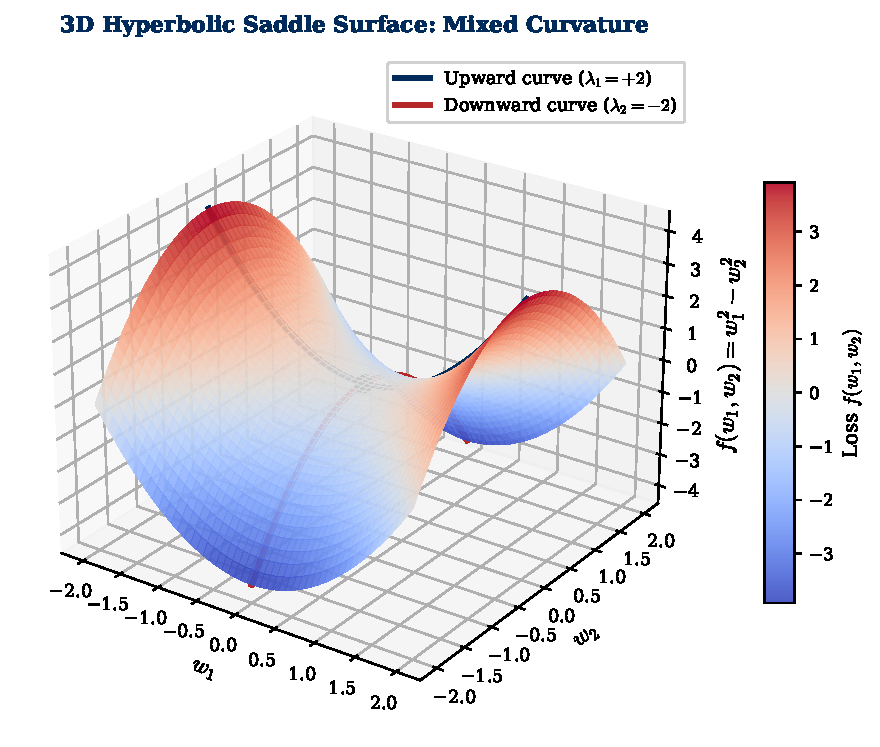
\includegraphics[width=\linewidth]{figures/saddle_point_landscape.pdf}
  \caption{High-resolution 3D visualization of the hyperbolic saddle surface, illustrating mixed eigenvalues $\lambda_1 > 0$ and $\lambda_2 < 0$.}
  \label{fig:manim_saddle_point}
\end{minipage}
\end{figure}

Figures~\ref{fig:slide_saddle_point} and~\ref{fig:manim_saddle_point} illustrate a canonical hyperbolic saddle surface $f(w_1, w_2) = w_1^2 - w_2^2$. At the origin $(0, 0)$, the gradient is zero: $\nabla f = [2w_1, -2w_2]^\top = [0, 0]^\top$. The Hessian matrix is constant:
\begin{equation}
\mathbf{H} = \begin{bmatrix} 2 & 0 \\ 0 & -2 \end{bmatrix},
\end{equation}
yielding eigenvalues $\lambda_1 = +2 > 0$ (along the $w_1$ axis) and $\lambda_2 = -2 < 0$ (along the $w_2$ axis).

\subsection{Proliferation of saddle points in high dimensions (Dauphin et al., 2014)}
\label{sec:dauphin_saddle_points}

In popular machine learning discourse, a persistent misconception is that training deep neural networks fails because first-order gradient descent gets trapped in poor local minima.

In a landmark paper presented at NeurIPS 2014, Dauphin, Bengio et al.~\cite{dauphin2014identifying} disproved this hypothesis using random matrix theory and Bray-Dean statistical physics of high-dimensional non-convex glasses. They established that:
\begin{enumerate}
  \item In a $d$-dimensional parameter space ($d \sim 10^7$ to $10^{11}$ in modern deep learning), the probability that all $d$ random eigenvalues of the Hessian share the same positive sign scales asymptotically as:
  \begin{equation}
  \mathbb{P}(\mathbf{H} \succ 0) \propto \left(\frac{1}{2}\right)^d \approx 0.
  \label{eq:saddle_point_probability}
  \end{equation}
  For $d = 1000$, $(1/2)^{1000} \approx 10^{-301}$, which is physically zero. Therefore, almost all critical points encountered in deep architectures are \textbf{saddle points}, not local minima!
  \item High-loss critical points are overwhelmingly surrounded by directions of negative curvature ($\lambda_i < 0$), providing open escape paths. True local minima exist almost exclusively near the bottom of the loss landscape, where empirical risk is already low and model generalization is strong.
  \item However, because $\|\nabla f(\mathbf{w})\| \approx 0$ in the vicinity of a saddle point, standard first-order gradient descent decelerates dramatically, spending exponential time navigating plateau-like saddle neighborhoods unless escaping noise is injected.
\end{enumerate}

\subsection{Why we are rarely interested in the global optimum}
\label{sec:global_optimum_fallacy}

In modern statistical learning, a foundational insight overturns classical intuition:
\begin{center}
\textbf{\Large\color{politoNavy} ``We are rarely interested in the global optimum!''}
\end{center}

In classical convex optimization, the global minimum is the undisputed goal. In deep learning, however, searching for the absolute global minimum of the empirical risk $\hat{\risk}_N(\mathbf{w})$ is not merely unnecessary—it is actively hazardous:
\begin{enumerate}
  \item \textbf{Overparameterization and Memorization}: Modern deep networks contain vastly more parameters than training samples ($d \gg N$). A network with millions of parameters possesses sufficient capacity to achieve zero empirical loss ($\hat{\risk}_N(\mathbf{w}^*) = 0$) by memorizing every arbitrary training sample, including mislabeled instances and random noise.
  \item \textbf{Generalization Failure}: Reaching the absolute global minimum of empirical loss often drives parameters into extreme overfitted configurations. Because the training set $\mathcal{D}_N$ is merely a finite empirical sample from underlying distribution $P$, perfectly fitting $\mathcal{D}_N$ creates huge errors on unseen test data ($\risk(h_{\mathbf{w}^*}) \gg 0$).
  \item \textbf{Sub-optimal Local Basins Generalize Better}: Any reasonable local minimum that achieves low (but non-zero) loss and resides in a broad, well-behaved basin yields vastly superior generalization compared to the degenerate empirical global optimum.
\end{enumerate}

\subsection{Flat vs. sharp minima: Hessian spectrum and test distribution generalization}
\label{sec:flat_vs_sharp_minima}

To formalize why certain local minima generalize while others overfit, optimization theory examines the \textbf{spectral flatness} of the loss basin (Hochreiter \& Schmidhuber~\cite{hochreiter1997flat}; Keskar et al.~\cite{keskar2017large}):

\begin{figure}[htbp]
\centering
\resizebox{0.96\linewidth}{!}{%
\begin{tikzpicture}
  % Panel A: Flat vs Sharp Minima under Distribution Shift
  \begin{axis}[
    name=plot1,
    width=8.8cm, height=6.2cm,
    axis lines=left,
    xlabel={Parameter $\mathbf{w}$},
    ylabel={Loss $\mathcal{L}(\mathbf{w})$},
    xmin=0.5, xmax=8.4,
    ymin=0, ymax=3.3,
    ticks=none,
    title={\textbf{(a) Generalization gap under distribution shift}},
    title style={font=\footnotesize, at={(0.5,1.05)}, anchor=south}
  ]
    % Train loss
    \addplot[very thick, politoNavy, domain=1.0:6.5, samples=150] 
      {1.8 + 0.05*(x-4.0)^2 - 1.5*exp(-(x-2.0)^2 / 0.10) - 1.2*exp(-(x-5.2)^2 / 1.5)}
      node[pos=1.0, right, font=\scriptsize\bfseries, text=politoNavy] {Train $\hat{\mathcal{R}}_N$};

    % Test loss (shifted by Delta w = 0.4)
    \addplot[very thick, examred, dashed, domain=1.0:6.5, samples=150] 
      {1.8 + 0.05*(x-0.4-4.0)^2 - 1.5*exp(-(x-0.4-2.0)^2 / 0.10) - 1.2*exp(-(x-0.4-5.2)^2 / 1.5)}
      node[pos=1.0, right, font=\scriptsize\bfseries, text=examred] {Test $\mathcal{R}_{\mathrm{test}}$};

    % Sharp minimum point at x = 2.0
    \draw[dotted, thick, gray!70] (axis cs:2.0, 0) -- (axis cs:2.0, 1.78);
    \fill[politoNavy] (axis cs:2.0, 0.50) circle (2.2pt);
    \fill[examred] (axis cs:2.0, 1.78) circle (2.2pt);
    \node[above left, font=\scriptsize\bfseries, text=politoNavy] at (axis cs:2.0, 0.50) {$\mathbf{w}^*_{\mathrm{sharp}}$};
    
    % Vertical gap at sharp minimum
    \draw[{Stealth[length=4pt]}-{Stealth[length=4pt]}, thick, examred] (axis cs:2.0, 0.56) -- (axis cs:2.0, 1.72);
    \node[right, font=\scriptsize\bfseries, text=examred, align=left] at (axis cs:2.05, 1.15) {Large gap\\(overfitting)};

    % Flat minimum point at x = 5.2
    \draw[dotted, thick, gray!70] (axis cs:5.2, 0) -- (axis cs:5.2, 0.75);
    \fill[politoNavy] (axis cs:5.2, 0.67) circle (2.2pt);
    \fill[examred] (axis cs:5.2, 0.75) circle (2.2pt);
    \node[below, font=\scriptsize\bfseries, text=politoNavy] at (axis cs:5.2, 0.58) {$\mathbf{w}^*_{\mathrm{flat}}$};

    % Small gap at flat minimum
    \draw[{Stealth[length=3pt]}-{Stealth[length=3pt]}, thick, intuitiongreen] (axis cs:5.2, 0.69) -- (axis cs:5.2, 0.73);
    \node[above, font=\scriptsize\bfseries, text=intuitiongreen, align=center] at (axis cs:5.3, 1.20) {Small gap\\(generalizes)};

    % Basin labels
    \node[above, font=\scriptsize\bfseries, text=politoNavy] at (axis cs:2.0, 2.7) {Sharp Minimum};
    \node[above, font=\scriptsize\bfseries, text=politoNavy] at (axis cs:5.2, 2.7) {Flat Basin};
  \end{axis}

  % Panel B: Escaping Sharp Traps via Momentum and Stochastic Noise
  \begin{axis}[
    name=plot2,
    at={($(plot1.east)+(1.8cm, 0)$)},
    anchor=west,
    width=8.8cm, height=6.2cm,
    axis lines=left,
    xlabel={Parameter $\mathbf{w}$},
    ylabel={Loss $\mathcal{L}(\mathbf{w})$},
    xmin=0.5, xmax=8.4,
    ymin=0, ymax=3.3,
    ticks=none,
    title={\textbf{(b) Escaping sharp traps via momentum \& SGD noise}},
    title style={font=\footnotesize, at={(0.5,1.05)}, anchor=south}
  ]
    % Loss landscape
    \addplot[very thick, politoNavy, domain=1.0:6.5, samples=150] 
      {1.8 + 0.05*(x-4.0)^2 - 1.5*exp(-(x-2.0)^2 / 0.10) - 1.2*exp(-(x-5.2)^2 / 1.5)}
      node[pos=1.0, right, font=\scriptsize\bfseries, text=politoNavy] {Loss $f(\mathbf{w})$};

    % Initial point w0
    \coordinate (w0) at (axis cs:1.3, 1.75);
    \shade[ball color=examred] (w0) circle (4pt) node[above left, font=\scriptsize\bfseries, text=examred] {$\mathbf{w}_0$};

    % GD path into sharp trap
    \draw[-{Stealth[length=4pt]}, thick, gray!80, dashed] (w0) to[out=-50, in=170] (axis cs:2.0, 0.52);
    \fill[gray!80] (axis cs:2.0, 0.50) circle (2.5pt);
    \node[above, font=\scriptsize\bfseries, text=gray!80, align=center] at (axis cs:1.6, 0.55) {GD stalls\\in trap};

    % Momentum trajectory flowing along the curve and overcoming barrier
    \draw[-{Stealth[length=5pt]}, very thick, deepdiveTeal] (axis cs:2.0, 0.54) 
      to[out=70, in=185] (axis cs:3.5, 1.68)
      to[out=5, in=170] (axis cs:4.4, 1.15)
      to[out=-10, in=180] (axis cs:5.2, 0.70);
    
    % Ball at the barrier
    \shade[ball color=deepdiveTeal] (axis cs:3.5, 1.70) circle (4pt);
    \node[above, font=\scriptsize\bfseries, text=deepdiveTeal, align=center] at (axis cs:3.5, 2.05) {Velocity $\mathbf{v}$ carries\\over barrier};

    % Ball in flat basin
    \shade[ball color=intuitiongreen] (axis cs:5.2, 0.67) circle (4pt);
    \node[below, font=\scriptsize\bfseries, text=intuitiongreen, align=center] at (axis cs:5.2, 0.55) {Wide Flat Basin\\(generalizes)};

    % Basin labels
    \node[above, font=\scriptsize\bfseries, text=politoNavy] at (axis cs:2.0, 2.7) {Sharp Trap};
    \node[above, font=\scriptsize\bfseries, text=politoNavy] at (axis cs:5.2, 2.7) {Flat Basin};
  \end{axis}
\end{tikzpicture}%
}
\caption{The geometry of generalization in non-convex optimization. (a) Under empirical-to-test distribution shift $\Delta \mathbf{w}$, evaluating a sharp minimum $\mathbf{w}^*_{\mathrm{sharp}}$ (large Hessian eigenvalues $\lambda_i \gg 0$) causes test loss to explode ($\Delta \mathcal{R} \gg 0$), resulting in severe overfitting. Conversely, a flat minimum $\mathbf{w}^*_{\mathrm{flat}}$ (small Hessian eigenvalues $\lambda_i \approx 0$) experiences negligible loss increase, ensuring robust generalization. (b) Standard gradient descent readily gets trapped in narrow, high-loss sharp valleys, whereas momentum velocity $\mathbf{v}$ and stochastic mini-batch noise provide the kinetic energy to escape barriers and settle into wide, flat basins.}
\label{fig:flat_vs_sharp_minima}
\end{figure}

As demonstrated in Figure~\ref{fig:flat_vs_sharp_minima}:
\begin{itemize}
  \item \textbf{Sharp Minima ($\lambda_{\max} \gg 0$)}: Characterized by narrow, steep ravines. Because the empirical training distribution $\hat{P}$ differs slightly from the true underlying distribution $P$, the test loss landscape is shifted horizontally by some small displacement $\Delta \mathbf{w}$. In a sharp well, moving $\mathbf{w}^*_{\text{sharp}} + \Delta \mathbf{w}$ catapults the loss value up the steep canyon wall, causing a catastrophic generalization gap.
  \item \textbf{Flat Minima ($\lambda_{\max} \approx 0$)}: Characterized by wide, gentle valleys. Under the exact same parameter displacement $\Delta \mathbf{w}$, the test loss remains virtually unchanged: $\mathcal{R}_{\text{test}}(\mathbf{w}^*_{\text{flat}} + \Delta \mathbf{w}) \approx \hat{\mathcal{R}}_N(\mathbf{w}^*_{\text{flat}})$. Flat minima are inherently robust to distribution shift and parameter quantization.
  \item \textbf{Kinetic Escape}: While standard batch gradient descent easily gets trapped in steep, non-generalizing local basins, momentum velocity $\mathbf{v}$ and stochastic mini-batch noise $\boldsymbol{\xi}_t$ act as dynamic perturbations that kick parameters over low barriers, naturally filtering out sharp wells in favor of expansive flat basins.
\end{itemize}

\subsection{The imperative for numerical optimization even on convex problems}
\label{sec:convex_problems_numerical_optimization}

This raises an essential theoretical question: \emph{if a machine learning problem is convex and possesses an exact analytical solution, why do we still use iterative gradient descent?}

\begin{enumerate}
  \item \textbf{Computational Complexity and Memory Scaling in OLS}:
    For linear regression, the closed-form normal equations yield $\mathbf{w}^* = (\mathbf{X}^\top \mathbf{X})^{-1}\mathbf{X}^\top \mathbf{y}$. 
    Forming the Gram matrix $\mathbf{X}^\top \mathbf{X}$ requires $\mathcal{O}(N d^2)$ operations, and inverting it via Cholesky or LU decomposition requires $\mathcal{O}(d^3)$ arithmetic operations and $\mathcal{O}(d^2)$ memory storage.
    When $d = 10^5$ (common in text, genomic, or computer vision representations), storing $d \times d$ floating-point matrices requires $40\text{ GB}$ of RAM, and computing $d^3 = 10^{15}$ operations is intractable.
    In contrast, first-order gradient descent scales as $\mathcal{O}(Nd)$ per iteration and requires only $\mathcal{O}(d)$ memory, enabling optimization on commodity hardware.
  \item \textbf{Numerical Stability and Ill-Conditioning}:
    When features are collinear, the condition number $\kappa(\mathbf{X}^\top \mathbf{X}) = (\kappa(\mathbf{X}))^2$ is squared! Direct matrix inversion suffers from catastrophic floating-point cancellation. Iterative gradient descent (especially when regularized via weight decay or early stopping) provides vastly superior numerical stability.
  \item \textbf{Non-Existence of Closed Forms in Generalized Linear Models}:
    As proven in Section~\ref{sec:no_closed_form_solution}, composing linear predictors with non-linear sigmoid or softmax links destroys linear algebra solvability. For logistic regression, closed-form inversion is mathematically impossible, leaving iterative optimization as the sole viable path.
\end{enumerate}

---

\section{Stochastic gradient descent (SGD), mini-batch dynamics, and large-scale learning bounds}
\label{sec:sgd_and_minibatch}

The empirical risk objective $\hat{\risk}_n(\boldsymbol{\theta})$ is defined as an arithmetic mean across $n$ training observations:
\begin{equation}
\ell(\boldsymbol{\theta}) = \frac{1}{n} \sum_{i=1}^n \hat{\ell}_i(\boldsymbol{\theta}), \quad \text{where } \hat{\ell}_i(\boldsymbol{\theta}) \equiv \ell(f_{\boldsymbol{\theta}}(\mathbf{x}_i), y_i).
\label{eq:sum_loss_structure}
\end{equation}
By linearity of differentiation, computing the full batch gradient requires evaluating:
\begin{equation}
\nabla \ell(\boldsymbol{\theta}) = \frac{1}{n} \sum_{i=1}^n \nabla \hat{\ell}_i(\boldsymbol{\theta}).
\label{eq:full_batch_gradient}
\end{equation}

\subsection{The two computational bottlenecks of gradient descent}
\label{sec:two_bottlenecks_gd}

Equation~\eqref{eq:full_batch_gradient} exposes the \textbf{two fundamental bottlenecks} that render full-batch gradient descent impractical for contemporary machine learning:
\begin{enumerate}
  \item \textbf{Bottleneck 1: Number of examples $n$}. In modern datasets (ImageNet, web corpora), $n$ ranges from $10^6$ to $10^{12}$. Evaluating all $n$ forward-backward passes to execute a single parameter step takes hours or days, stalling progress completely.
  \item \textbf{Bottleneck 2: Number of parameters $d$}. Neural networks contain millions to billions of parameters ($d \sim 10^7$--$10^{11}$). Storing, communicating, and computing gradients across $d$ dimensions per sample magnifies computational overhead.
\end{enumerate}

\subsection{Batch vs. stochastic vs. mini-batch estimators and the MNIST speedup}
\label{sec:gradient_estimators_taxonomy}

To break the dataset size bottleneck $n$, we approximate the full summation over training set $\mathcal{T}$ ($|\mathcal{T}| = n$) by evaluating the gradient over a small, representative, uniformly drawn subset $\mathcal{B} \subset \mathcal{T}$ of cardinality $m \ll n$ (termed a \textbf{mini-batch}):
\begin{equation}
\frac{1}{m} \sum_{i \in \mathcal{B}} \nabla \hat{\ell}_i(\boldsymbol{\theta}) \approx \frac{1}{n} \sum_{i \in \mathcal{T}} \nabla \hat{\ell}_i(\boldsymbol{\theta}).
\label{eq:minibatch_approximation}
\end{equation}

\paragraph{A concrete benchmark speedup calculation: MNIST.}
To appreciate the computational advantage concretely, consider the canonical MNIST handwritten digit benchmark:
\begin{itemize}[noitemsep]
  \item Full training set size: $n = 60{,}000$ images.
  \item Mini-batch size: $m = 10$ images.
  \item Speedup factor per gradient update:
  \begin{equation}
  \text{Speedup} = \frac{n}{m} = \frac{60{,}000}{10} = \mathbf{6{,}000 \times \text{ faster per step!}}
  \end{equation}
\end{itemize}
In the time full-batch GD takes to evaluate a single update, mini-batch SGD executes 6,000 parameter updates, making massive progress across the loss terrain.

\subsection{Algorithmic cycle and epoch progression}
\label{sec:algorithmic_cycle_epochs}

The procedural execution of mini-batch stochastic gradient descent proceeds cyclically:
\begin{enumerate}
  \item \textbf{Initialization}: Initialize parameter vector $\boldsymbol{\theta}^{(0)} \in \R^d$ (e.g., via He or Xavier initialization).
  \item \textbf{Mini-Batch Sampling}: Uniformly sample a mini-batch $\mathcal{B} \subset \mathcal{T}$ of size $m$.
  \item \textbf{Downhill Parameter Step}: Update parameters in the negative gradient direction (optionally incorporating momentum velocity):
    \begin{equation}
    \boldsymbol{\theta} \leftarrow \boldsymbol{\theta} - \alpha \nabla \ell_{\boldsymbol{\theta}}(\mathcal{B}).
    \label{eq:minibatch_algorithmic_step}
    \end{equation}
  \item \textbf{Recurrence and Epoch Completion}: Repeat steps 2--3. When accumulated mini-batches exhaustively cover the entire training set $\mathcal{T}$, one \textbf{epoch} is completed. Training iterates across multiple epochs until validation performance plateaus.
\end{enumerate}

\begin{remark}[Constant Update Cost]
A crucial property is that the update cost per iteration is $\mathcal{O}(m \cdot d)$, which is \textbf{strictly constant regardless of the total size of dataset $\mathcal{T}$}. This invariance enables deep learning algorithms to scale gracefully to virtually infinite streaming datasets.
\end{remark}

\subsection{Statistical properties: Unbiasedness, variance scaling, and steady-state oscillations}
\label{sec:minibatch_statistics}

We formalize the statistical properties of the stochastic gradient estimator:

\paragraph{1. Unbiasedness.}
Let indices in mini-batch $\mathcal{B}$ be drawn uniformly at random without replacement from $\{1, \dots, n\}$. The expected value of the estimator is:
\begin{equation}
\mathbb{E}_{\mathcal{B}}\left[ \frac{1}{m} \sum_{i \in \mathcal{B}} \nabla \hat{\ell}_i(\boldsymbol{\theta}) \right] = \frac{1}{m} \sum_{i \in \mathcal{B}} \mathbb{E}\left[ \nabla \hat{\ell}_i(\boldsymbol{\theta}) \right] = \frac{1}{m} \cdot m \cdot \left( \frac{1}{n} \sum_{k=1}^n \nabla \hat{\ell}_k(\boldsymbol{\theta}) \right) = \nabla \ell(\boldsymbol{\theta}).
\label{eq:unbiased_gradient}
\end{equation}
The mini-batch gradient is an \textbf{unbiased estimator} of the true full-batch gradient.

\paragraph{2. Variance reduction via batch size $m$.}
Let $\sigma^2 = \frac{1}{n} \sum_{i=1}^n \|\nabla \hat{\ell}_i(\boldsymbol{\theta}) - \nabla \ell(\boldsymbol{\theta})\|_2^2$ denote sample gradient variance. The covariance of the mini-batch estimator satisfies:
\begin{equation}
\mathbb{E}\left[ \left\| \frac{1}{m} \sum_{i \in \mathcal{B}} \nabla \hat{\ell}_i(\boldsymbol{\theta}) - \nabla \ell(\boldsymbol{\theta}) \right\|_2^2 \right] = \frac{\sigma^2}{m} \left( \frac{n - m}{n - 1} \right) \approx \frac{\sigma^2}{m}.
\label{eq:minibatch_variance_reduction}
\end{equation}
Variance contracts as $\mathcal{O}(1/m)$, while computational cost scales as $\mathcal{O}(m)$. Due to the square-root law of diminishing returns ($\operatorname{StdDev} \propto 1/\sqrt{m}$), increasing batch size from $m = 32$ to $1024$ increases compute by $32\times$, but only reduces noise by $\sqrt{32} \approx 5.65\times$. Hence, moderate batch sizes ($32 \le m \le 256$) offer the optimal trade-off between parallel throughput and stochastic exploration.

\begin{figure}[htbp]
\centering
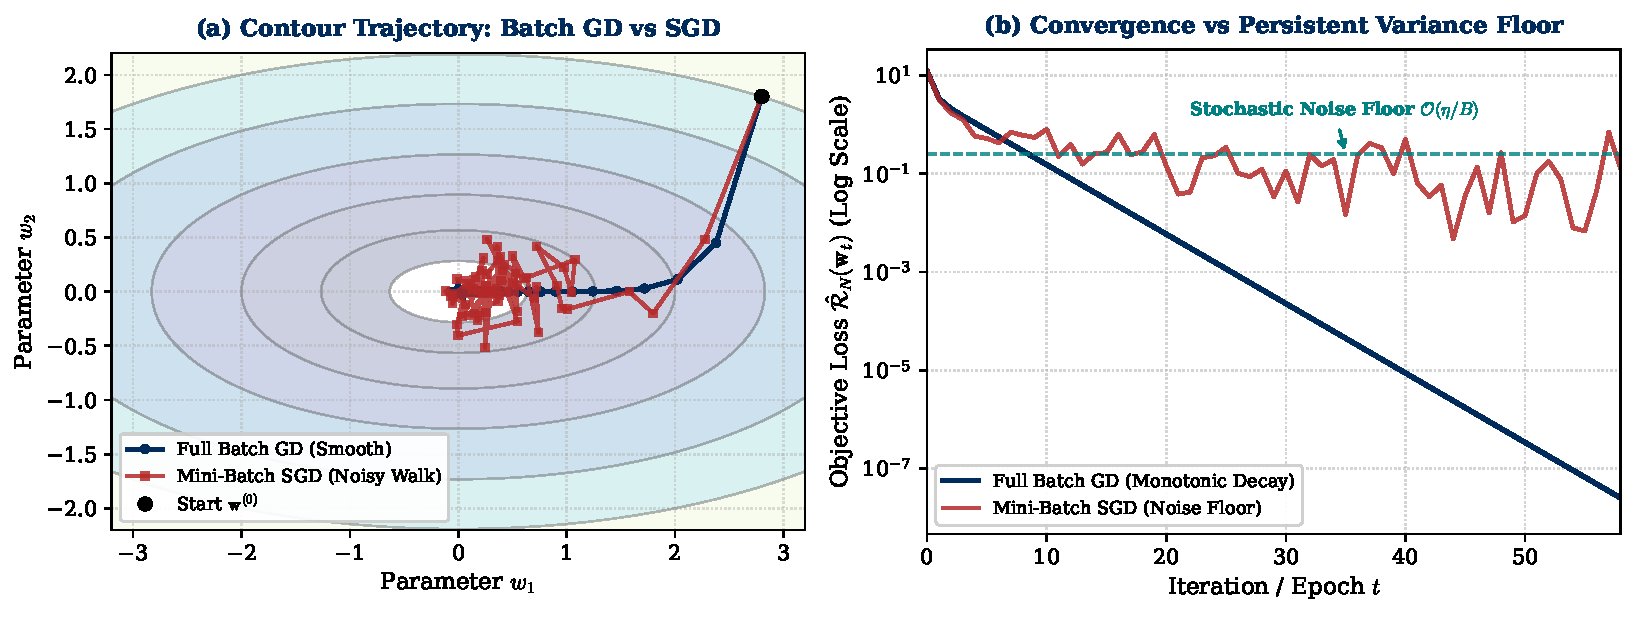
\includegraphics[width=0.95\linewidth]{figures/sgd_oscillations_dynamics.pdf}
\caption{Stochastic gradient descent dynamics: (Left) Contour trajectory showing the noisy Brownian-like walk around the loss minimum without exact stationary convergence; (Right) Parameter weight evolution over epochs on a logarithmic scale, illustrating rapid initial progress followed by persistent steady-state stochastic variance fluctuations induced by random data subsampling.}
\label{fig:slide_minibatch_dynamics}
\end{figure}

\paragraph{Why SGD does not stop at the minimum.}
As illustrated in Figure~\ref{fig:slide_minibatch_dynamics}, a defining hallmark of SGD is that \textbf{it does not halt at the minimum}:
\begin{equation}
\lim_{t \to \infty} \mathbb{E}\left[ \|\boldsymbol{\theta}_t - \boldsymbol{\theta}^*\|_2^2 \right] \approx \mathcal{O}(\alpha \sigma^2).
\end{equation}
Even when the true gradient vanishes at the minimizer ($\nabla \ell(\boldsymbol{\theta}^*) = \mathbf{0}$), individual sample gradients $\nabla \hat{\ell}_i(\boldsymbol{\theta}^*)$ do not vanish! Consequently, mini-batch gradients retain stochastic noise, causing parameters to wander indefinitely in a steady-state covariance cloud around $\boldsymbol{\theta}^*$.

\subsection{Robbins-Monro convergence conditions for stochastic optimization}
\label{sec:robbins_monro}

To extinguish persistent stochastic oscillations and guarantee almost sure convergence to a stationary point ($\lim_{t \to \infty} \boldsymbol{\theta}_t = \boldsymbol{\theta}^*$), the learning rate sequence $\{\alpha_t\}_{t=1}^\infty$ must be decayed.

In their foundational 1951 paper on stochastic approximation, Herbert Robbins and Sutton Monro~\cite{robbins1951stochastic} established the necessary and sufficient conditions:
\begin{equation}
\sum_{t=1}^\infty \alpha_t = \infty \quad \text{and} \quad \sum_{t=1}^\infty \alpha_t^2 < \infty.
\label{eq:robbins_monro_conditions}
\end{equation}
\begin{itemize}[noitemsep]
  \item \textbf{Condition 1 ($\sum \alpha_t = \infty$)}: Guarantees infinite exploration horizon. The cumulative distance parameters can travel is unbounded, ensuring the optimizer never stalls before reaching the minimum basin.
  \item \textbf{Condition 2 ($\sum \alpha_t^2 < \infty$)}: Guarantees variance extinction. Because cumulative error variance accumulates as $\sum \alpha_t^2 \sigma^2 < \infty$, stochastic fluctuations vanish asymptotically at $\boldsymbol{\theta}^*$.
\end{itemize}

\subsection{Asymptotic upper bounds for large-scale learning (Bottou \& Bousquet, 2008)}
\label{sec:bottou_bousquet_bounds}

The seminal theoretical framework of Léon Bottou and Olivier Bousquet~\cite{bottou2008tradeoffs} (NeurIPS 2008, \emph{``The Tradeoffs of Large Scale Learning''}) rigorously demonstrates why SGD achieves superior generalization compared to full-batch GD under bounded computational budgets.

Consider a convex learning problem with training set size $n$, parameter dimension $d$, and objective condition number $\kappa$. We seek to achieve target accuracy $\rho > 0$ on excess true risk:
\begin{equation}
\left| \ell(h_{\boldsymbol{\theta}}) - \ell(f^*) \right| < \rho,
\label{eq:excess_risk_target}
\end{equation}
where $\ell(h_{\boldsymbol{\theta}})$ is the expected risk of the learned hypothesis, and $\ell(f^*)$ is the Bayes optimal risk.

\begin{table}[htbp]
\centering
\caption{Asymptotic upper bounds for reaching excess risk $\rho$ on convex problems (Bottou \& Bousquet, NeurIPS 2008). Here $\kappa$ and $\nu$ are constants governing objective conditioning and gradient variance.}
\label{tab:bottou_bousquet_bounds}
\begin{tabularx}{0.92\textwidth}{lXX}
\toprule
\textbf{Optimization Algorithm} & \textbf{Computational Cost per Iteration} & \textbf{Iterations to Reach Target Error $\rho$} \\
\midrule
Full Batch Gradient Descent (GD) & $\mathcal{O}(n \cdot d)$ & $\mathcal{O}\left(\kappa \log \frac{1}{\rho}\right)$ \\
\addlinespace
Stochastic Gradient Descent (SGD) & $\mathcal{O}(d)$ & $\frac{\nu \kappa^2}{\rho} + o\left(\frac{1}{\rho}\right)$ \\
\bottomrule
\end{tabularx}
\end{table}

\paragraph{The profound theoretical implication: Total computational cost.}
Evaluating the total computational work required to reach accuracy $\rho$:
\begin{align}
\text{Total Work}_{\text{GD}} &= \mathcal{O}(nd) \times \mathcal{O}\left(\kappa \log \frac{1}{\rho}\right) = \mathcal{O}\left( n \cdot d \cdot \kappa \log \frac{1}{\rho} \right), \label{eq:total_work_gd} \\
\text{Total Work}_{\text{SGD}} &= \mathcal{O}(d) \times \left( \frac{\nu \kappa^2}{\rho} + o\left(\frac{1}{\rho}\right) \right) = \mathcal{O}\left( \frac{d \cdot \nu \kappa^2}{\rho} \right). \label{eq:total_work_sgd}
\end{align}

\begin{examinsight}[Oral Exam Milestone: Why SGD Generalizes Better]
Observe the fundamental distinction between Equations~\eqref{eq:total_work_gd} and~\eqref{eq:total_work_sgd}:
\begin{center}
\textbf{The total computational cost of SGD does NOT depend on the number of training examples $n$!}
\end{center}
In large-scale machine learning where computation time is limited:
\begin{itemize}[noitemsep]
  \item \textbf{Full Batch GD} spends vast computational resources computing ultra-precise gradients over a fixed, finite dataset $\mathcal{D}_n$, driving empirical training error to zero but over-fitting sample noise.
  \item \textbf{SGD} takes cheap, noisy steps that each touch new, unvisited samples. For a fixed computational budget of floating-point operations (FLOPs), SGD processes orders of magnitude more distinct data samples from distribution $P$.
\end{itemize}
Because statistical generalization error is bounded by the total amount of unique data processed rather than optimization precision on a small set, \textbf{SGD achieves strictly superior generalization error (true risk)}!
\end{examinsight}

\subsection{Practical considerations in modern deep learning SGD}
\label{sec:practical_sgd_deep_learning}

To conclude the optimization framework, we synthesize five foundational practical principles for deploying SGD in contemporary neural networks:

\begin{enumerate}
  \item \textbf{Data Shuffling to Eliminate Ordering Bias}:
    Mini-batches must be drawn by randomly shuffling the dataset at the start of every epoch. If data exhibits sequential correlation (e.g., all class~1 digits grouped together), sequential mini-batches will violently drag parameters toward class~1, causing catastrophic forgetting of preceding classes and inducing cyclic optimization orbits.
  \item \textbf{Hardware Parallelization and SIMD Efficiency}:
    While pure SGD ($m = 1$) is optimal in theory, single-sample operations fail to exploit GPU parallelism. Mini-batch sizes $m \in \{32, 64, 128, 256, 512\}$ are chosen to match GPU Streaming Multiprocessor warp sizes and saturate Tensor Core matrix multiplication units (GEMM).
  \item \textbf{Two-Phase Optimization Dynamics}:
    SGD exhibits an asymmetric temporal profile: \textbf{remarkably rapid initial progress} in early epochs as parameters drop down steep macro-gradients into low-loss valleys, followed by \textbf{slow asymptotic fine-tuning} where parameter wanderings are dominated by gradient variance.
  \item \textbf{Implicit Regularization of Small Mini-Batches}:
    Small mini-batches inject high stochastic gradient noise ($\propto \sigma^2 / m$). This noise acts as an implicit regularizer, preventing parameters from settling into sharp overfitted minima and nudging trajectories into wide flat basins. However, because variance is high, practitioners must reduce the learning rate $\alpha$ (or apply linear learning rate scaling $\alpha \propto m$) to preserve numerical stability.
  \item \textbf{The Practitioner's Fundamental Maxim}:
    This crystallizes the ultimate operational rule of deep learning optimization:
    \begin{center}
    \textbf{\large\color{politoNavy} ``SGD can find a low value of the loss quickly enough to be useful, even if it's not a minimum.''}
    \end{center}
    In real-world engineering, achieving an exact stationary point ($\nabla \ell = \mathbf{0}$) is neither required nor desirable. Finding a robust, flat basin with low empirical loss within practical time constraints delivers state-of-the-art generalization.
\end{enumerate}

\clearpage
\enlargethispage{\baselineskip}
\subsection{Systematic comparison of gradient descent paradigms}
\label{sec:systematic_comparison}

Table~\ref{tab:gradient_comparison} synthesizes the mathematical, computational, and algorithmic trade-offs across the gradient descent family.

\begin{table}[htbp]
\centering
\small
\renewcommand{\arraystretch}{0.90}
\caption{Systematic comparison of Batch Gradient Descent, Stochastic Gradient Descent (SGD), and Mini-Batch SGD.}
\label{tab:gradient_comparison}
\begin{tabularx}{\textwidth}{lXXX}
\toprule
\textbf{Property} & \textbf{Batch Gradient Descent} & \textbf{Stochastic GD (SGD)} & \textbf{Mini-Batch SGD} \\

\midrule
\textbf{Batch Size $B$} & $B = n$ (full dataset) & $B = 1$ (single sample) & $1 < B < n$ (typically $32$--$512$) \\
\textbf{Cost per Step} & $\mathcal{O}(n \cdot d)$ & $\mathcal{O}(d)$ & $\mathcal{O}(B \cdot d)$ \\
\textbf{Gradient Variance} & Zero (deterministic) & High ($\sigma^2$) & Controlled ($\sigma^2 / B$) \\
\textbf{Convergence Path} & Monotonic \& smooth & Erratic \& oscillatory & Controlled variance cloud \\
\textbf{Hardware Affinity} & Memory bound on large $n$ & Poor GPU SIMD usage & Highly optimized for GPU BLAS \\
\textbf{Saddle Point Escape} & Vulnerable to stall & High escape ability & Strong escape via noise \\
\textbf{Scaling with $n$} & Total work scales with $n$ & Total work independent of $n$ & Total work independent of $n$ \\
\textbf{Generalization} & Prone to sharp traps & Excellent (flat basins) & Optimal (balanced noise) \\
\bottomrule
\end{tabularx}
\end{table}

\subsection{Chapter synthesis and roadmap to representation learning}
\label{sec:chapter3_synthesis}

Across Chapters~1 through~3, we have traversed the foundational triad of statistical machine learning:
\begin{enumerate}[noitemsep,topsep=2pt,parsep=0pt,partopsep=0pt]
  \item \textbf{Statistical foundations (Chapter~1)}: Defining learning paradigms, hypothesis spaces, and the fundamental trade-off between empirical risk and true risk.
  \item \textbf{Decision-theoretic limits (Chapter~2)}: Formulating the Bayes optimal predictor, irreducible noise, and the estimation/approximation trade-off governing model capacity.
  \item \textbf{Loss geometry and optimization (Chapter~3)}: Moving from the non-convex pathologies of squared error in classification to cross-entropy, and replacing intractable analytical matrix inversions with first-order iterative methods (GD, Momentum, and Mini-batch SGD).
\end{enumerate}

The decisive realization uniting this theoretical arc is that \textbf{optimization in machine learning is subservient to generalization}. Unlike classical numerical analysis, where reaching an exact critical point ($\nabla \ell = \mathbf{0}$) is paramount, deep learning exploits stochastic gradient noise, momentum dynamics, and early stopping as implicit regularizers that bias trajectories away from sharp overfitted traps and toward wide, flat basins with superior test performance.

However, all models examined thus far have relied on \textbf{fixed linear representations} $\mathbf{w}^\top \mathbf{x} + b$. Even when paired with cross-entropy and trained via mini-batch SGD, a linear hyperplane cannot separate nonlinearly distributed data (such as the classical XOR problem or complex perceptual manifolds). To transcend this expressivity bottleneck, machine learning diverges into two great paradigms:
\begin{itemize}[noitemsep,topsep=2pt,parsep=0pt,partopsep=0pt]
  \item \textbf{Implicit feature spaces (Kernel Methods and SVMs)}: Projecting inputs into high- (or infinite-) dimensional Hilbert spaces via the kernel trick while retaining convex dual optimization.
  \item \textbf{Explicit hierarchical representations (Deep Neural Networks)}: Learning parameterized feature transformations end-to-end via composite nonlinear layers, where optimization gradients are propagated through intermediate representations using the chain rule (Backpropagation).
\end{itemize}
These representation learning paradigms form the core of the upcoming chapters.


